\documentclass{article}

\usepackage{hyperref}       % hyperlinks
\usepackage{url}            % simple URL typesetting
\usepackage{booktabs}       % professional-quality tables
\usepackage{amsfonts}       % blackboard math symbols
\usepackage{nicefrac}       % compact symbols for 1/2, etc.
\usepackage{microtype}      % microtypography

\usepackage{graphicx}
\usepackage{amsmath}
\usepackage{amssymb}
\usepackage{dsfont}
\usepackage[backend=biber, bibencoding=utf8, sorting=none]{biblatex}
\usepackage{inputenc}

\usepackage{fullpage}
\usepackage{float}
\usepackage[affil-it]{authblk}

\usepackage[colorinlistoftodos]{todonotes}

\DeclareMathOperator{\Tr}{Tr}
\DeclareMathOperator{\diag}{diag}
\DeclareMathOperator{\cor}{cor}

\newcommand{\beginsupplement}{%
        \setcounter{table}{0}
        \renewcommand{\thetable}{S\arabic{table}}%
        \setcounter{figure}{0}
        \renewcommand{\thefigure}{S\arabic{figure}}%
     }
     
     
\addbibresource{/home/brielin/Work/references/bib/bimmer_manuscript.bib}

\title{Phenome-scale causal discovery with
bidirectional mediated Mendelian randomization}

\author[1, 2]{Brielin C. Brown \thanks{bb2991@columbia.edu}}
\author[2, 3, 4]{David A. Knowles \thanks{dak2173@columbia.edu}}

\affil[1]{Data Science Institute, Columbia University, New York, NY}
\affil[2]{New York Genome Center, New York, NY}
\affil[3]{Department of Computer Science, Columbia University, New York, NY}
\affil[4]{Department of Systems Biology, Columbia University, New York, NY}

\date{}
\begin{document}
\maketitle

\begin{abstract}
Inference of directed biological networks from observational
genomics datasets is a long-standing challenge, with relevance to detecting
core genes under the omnigenic model of complex traits, finding pathways that
can be targeted for treatment, and understanding risk
factors for disease more broadly. However, interrogating the structure of networks is notoriously difficult
due to unmeasured confounding and reverse causation.
Despite this, modern population-scale biobanks  offer unprecedented opportunity to study biological networks
 because they can contain simultaneous measurements of
traits, molecular markers and genetic variation. Recently, Mendelian randomization
(MR) has received attention as a class of methods for inferring causal effects
in observational data by using genetic variants (SNPs) from genome-wide
association studies (GWAS) as instrumental variables. However,
MR methods must make strong assumptions that limit their
ability to be applied at the biobank-scale, including that
the SNP only effects the outcome through the exposure.
While some methods are able to relax this assumption, the application of MR
to complex traits remains challenging. Moreover MR estimates the
total causal effect (TCE) of the exposure on the outcome, which may be mediated by other factors.
The proliferation of phenome-scale datasets
allows researchers to simultaneously measure the effects of possible mediators,
in principle enabling the conversion of TCE estimates into causal direct effect (CDE) 
estimates.
Here, we introduce an approach called
bi-directional mediated Mendelian randomization (bimmer)
for inferring sparse networks of CDEs from phenome-scale
GWAS summary statistics.
Our approach has two parts. First, we perform bi-directional Mendelian randomization
between every pair of phenotypes using Egger regression with a
modified weighting scheme that reduces the influence of pleiotropic SNPs.
This gives an estimate of the TCE of each phenotype on every other.
Second, we perform a mediation analysis to convert the matrix
of TCEs into a sparse, directed network of CDEs.
We show that this conversion can be modeled as an sparse matrix inverse problem,
and introduce a novel algorithm for finding a sparse inverse to a partially-observed matrix.
We show in extensive simulations that our approach is able to learn causal
network structures even in the presence of non-causal genetic correlation and differential
power across phenotypes. We apply our method to 405 phenotypes from the UK Biobank,
inferring a graph with 2,826 edges
that often results in several paths between nodes adding together to form the TCE.
We demonstrate that learning the graph structure
allows us to both understand seemingly surprising effects, and also identify seemingly-significant
effects that lack network support. We use bimmer to identify several
sub-networks acting as densely connected hubs with correlated downstream effects, including a morphology
hub, a heart disease hub, a blood biomarker hub, and a red blood cell hub. These hubs yield
several insights and lend causal support to recent work elucidating the effect of testosterone
on lung function, and sex-hormone binding globulin on personality, among others.
Altogether, we conclude that bimmer is a powerful tool for interrogating complex trait networks
that allows researchers to conduct previously-difficult analyses.
\end{abstract}

\section{Introduction}
Recent developments in the understanding of complex-trait genetics have
lead to a call for increased study of biological networks~\cite{Boyle2017,Liu2019,Wray2018}.
However, interrogating the structure of networks is notoriously difficult,
owing to factors such as unmeasured confounding and reverse causation~\cite{Parsana2019}.
In spite of these challenges, modern population-scale biobanks 
offer unprecedented opportunity to study biological networks
 because they can contain simultaneous measurements of
traits, molecular markers and genetic variation~\cite{Sudlow2015,Nagai2017}.

Mendelian randomization (MR) has recently received increased attention as a class of methods
that can mitigate issues in causal inference
 by using genetic variants (SNPs) from genome-wide
association studies (GWAS) as instrumental variables to determine the effect
of an exposure (A) on an outcome (B). To estimate causal effects,
MR methods must make strong assumptions that limit their
ability to be applied at the biobank-scale. Perhaps the most
controversial assumption is that the SNP only effects B through A
(\textit{i.e.} there is no horizontal pleiotropy). Recent methods such as Egger
regression and the mode-based-estimator are able to relax this assumption, instead
assuming there is no correlated pleiotropy or modal pleiotopy, respectively~\cite{Bowden2015,Hartwig2017}.
Another approach, the latent causal variable (LCV) model, is able to detect causality
under arbitrarily-structured pleiotropy~\cite{OConnor2018}. However, the quantity that LCV
calculates is not interpretable as the causal effect size of A on B. Most MR studies
also presuppose the direction of effect, specifying one phenotype as the outcome and
the other as the exposure. This is sound when the outcome
is clearly biologically downstream of the exposure, but in some cases it is better
to learn the direction of the effect from the data.
Some researchers have instead used bi-directional MR~\cite{Timpson2011}, which tests for
and effect in each direction, or gwas-pw~\cite{Pickrell2016}, which infers the effect.
direction from the data.
However, the utility of these approaches for complex traits,
which might contain non-causal genetic correlation,
is questionable~\cite{OConnor2018}.

In mimicking a randomized controlled trial, MR estimates the
total causal effect (TCE) of A on B~\cite{Burgess2015}. This effect may be mediated by
any number of factors. The proliferation of phenome-scale datasets
allows researchers to simultaneously measure the effects of many possible mediators,
in principle enabling the conversion of TCE estimates into causal direct effect (CDE) 
estimates, which are not mediated by any other measured factor.
However, methods to enact this conversion are limited, either because they require complex
processing pipelines that limit their scope~\cite{Amar2019} or because they are
computationally intractable for graphs with more than a few nodes~\cite{Badsha2019}.
This raises another disadvantage of approaches such as LCV and gwas-pw. Assuming that either
A causes B or B causes A, but not both, is equivalent to assuming
that the underlying causal network
lacks cycles, which are thought to be an important part of real biological networks~\cite{Zhu2007}.

Here, we introduce an approach called
\emph{bi-directional mediated Mendelian randomization} (bimmer)
for inferring sparse networks of causal direct effects from phenome-scale
GWAS summary statistics.
Our approach has two parts. First, we perform bi-directional Mendelian randomization
between every pair of phenotypes using Egger regression with a
modified SNP selection and weighting scheme that reduces the
influence of pleiotropic SNPs.
This gives an estimate of the TCE of each phenotype on every other (Figure~\ref{figure0}a-b).
Second,
we perform a causal mediation analysis to convert the matrix
of total causal effects into a sparse, directed network of causal direct effects.
We show that this conversion can be modeled as an $L_1$-regularized matrix inverse problem,
drawing analogy to the graphical lasso~\cite{Friedman2007}, and introduce a new
algorithm for finding a sparse inverse to a partially-observed matrix called
\emph{inverse sparse regression} (inspre, Figure~\ref{figure0}b-c).
We show in extensive simulations that our approach is able to learn causal
 network structures even in the presence of non-causal genetic correlation.
We apply our method to $405$ phenotypes from the UK Biobank, finding thousands
 of direct causal effects, complex causal pathways, and concentrated sub-networks
 with correlated downstream effects.
 
\begin{figure}\label{figure0}
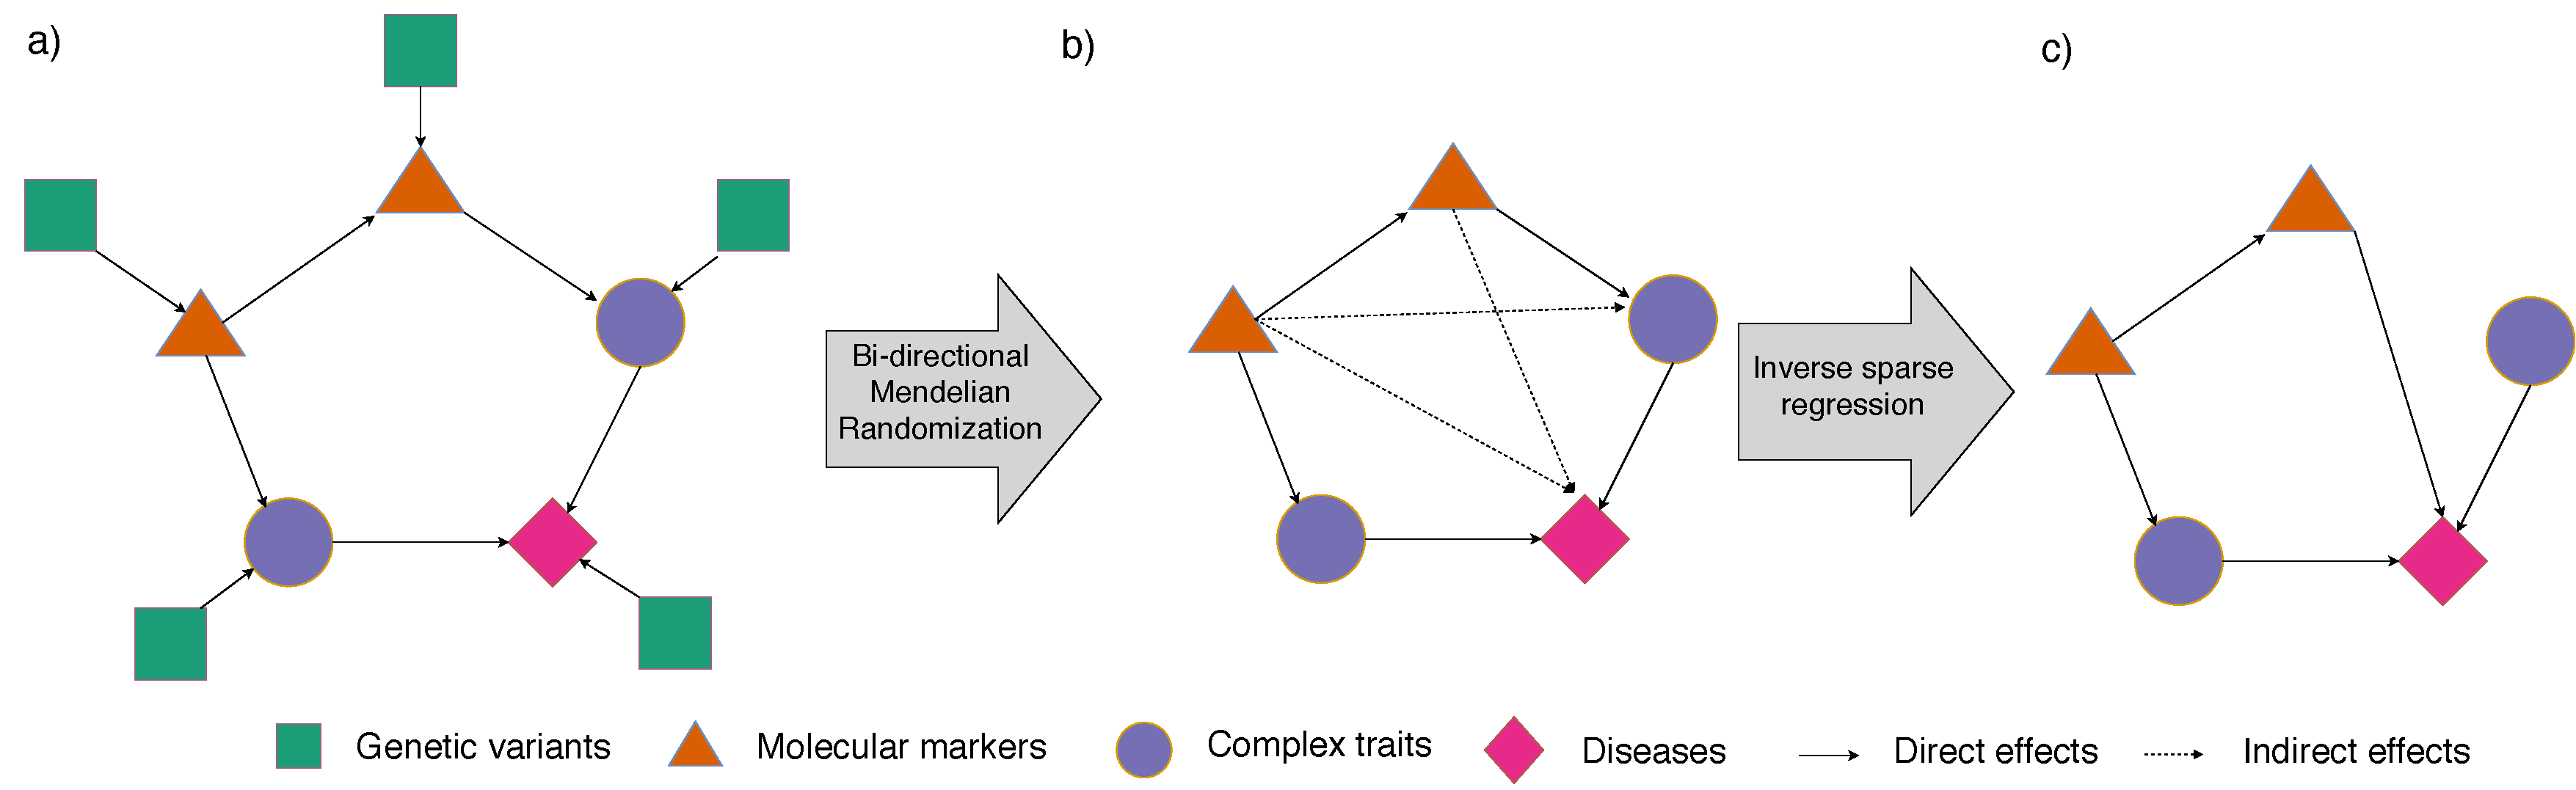
\includegraphics[width=\textwidth]{figures/bimmer_figure1.pdf}
\caption{Overview of the bimmer model. a) Modern biobanks contains measurements of genetic variants (green squares), molecular markers
(orange triangles), complex traits (purple circles) and diseases (pink diamonds). Genetic variants
affect these phenotypes which in turn affect each other. b) Bi-directional Mendelian randomization
estimates the total causal effect of the phenotypes on each other, which includes both
direct (solid arrow) and indirect (dashed arrow) effects. c) The direct effects can be
found by estimating a sparse approximate inverse to the matrix of total effects, a process we
call inverse sparse regression.}
\end{figure}
\todo{Replace with prettier picture highlighting possible pleiotropy, difference between true and 
estimated effects.}

\section{Results}
\subsection*{Overview of model}

We motivate our model by considering a linear dynamical system at equilibrium.
\todo{I dont think it's worth going into the multiple derivations. I never made them
completely rigorous and verified they really had non-overlapping assumptions.}
We model each phenotype as a function of 1) time-invariant genetic factors, 2)
time-invariant environmental factors, and 3) other phenotypes at the previous
time-point.
Assume we have $N$ individuals, $D$ phenotypes and $M$ SNPs,
with $Y_t$ the matrix of phenotypes indexed by time $t$, $X$ the genotype
matrix, $\beta$ the SNP effect matix and $\gamma$ a matrix of unknown
environmental effects. Let $R$ be the $D \times D$ matrix of
causal direct effects, with $R_{i, j}$ the CDE of phenotype $i$ on
phenotype $j$. We assume that phenotypes do not effect themselves ($R_{i,i} = 0$),
and that the network is sparse ($R$ has many entries that are $0$).
Our goal is to estimate $R$ given summary statistics
 for the association of the genotypes $X$ with the phenotypes measured when
 the system has reached equilibrium, $Y = Y_{t}$.
 Our trait model is
\begin{equation}
Y_{t+1} = Y_{t} R + X\beta + \gamma
\end{equation}
which converges to $Y = (X\beta + \gamma)(I-R)^{-1}$ if the largest eigenvalue
of $R$ has magnitude below 1.

Let $R^{TCE}$ be the matrix of TCE estimates from MR, with $R^{TCE}_{i,j}$ the total
causal effect of phenotype $i$ on phenotype $j$ and $S_{i,j}$ it's standard error.
We show in section~\ref{methods} that under this model,
\begin{equation}\label{r_cde_main}
R = I - R^{TCE^{-1}} D[1 / R^{TCE^{-1}}]
\end{equation}
where $D$ is an operator that sets all off-diagonal elements to 0, and $/$
represents element-wise division.

In practice, the matrix $R^{TCE}$ need not be well-conditioned or
 even invertible, leading
to challenges when calculating $R$ via~\eqref{r_cde_main}. Instead of calculating an exact
or psuedo-inverse, we exploit the assumption that the underlying
CDE matrix is sparse. Specifically, we seek matrices $U$ and $V$ such that $VU=I$, $U \approx R^{TCE}$ \todo{would it be better to set this up without $U$ and assume $V^{-1}$, then introduce the relaxation in the methods? brielin: I don't think so. I need something to use to refer to our approximation to the TCE later.}
and $V$ is sparse. We find them by solving the following constrained optimization problem,
\begin{equation} \label{opt_main}
\min_{\{U, V : VU = I\}} \frac{1}{2} ||W \circ (R^{TCE} - U)||_F^2 +
   \lambda \sum_{i\neq j}|V_{ij}|
\end{equation}
where $W = W_{i,j} = 1/S_{i,j}^2$ is a set of per-entry inverse variance weights,
and $\lambda$ is the $L_1$ shrinkage parameter~\cite{Friedman2007,Tishbirani1996}.
We refer to $U$ as bimmer shrunk estimates of the TCE, and
use $V \approx R^{TCE^{-1}}$ to solve~\eqref{r_cde_main}.
 Note that in this method, missing entries in $R^{TCE}$ can be accommodated simply
by setting their weights to 0. We use this property to our advantage in choosing the
regularization parameter. Specifically, we use a novel adaptation of Stability Approach
to Regularization Selection (StARS)~\cite{Liu2010} where we mask entries of the TCE
in order to induce variance in the estimated graph during cross-validation.
For complete details, see~\ref{methods}.

Some intuition for~\eqref{r_cde_main} can be gained by considering the problem
of estimating a matrix of partial correlations for a set of observed variables.
Analogous to the CDE, the partial correlation measures the degree to which two
variables are correlated while controlling for the effect of all other measured
variables. Given a matrix of observed (standard) correlations, $\Sigma$, the matrix of
partial correlations is $P = -D[\Sigma^{-1}]^{-1/2} \Sigma^{-1} D[\Sigma^{-1}]^{-1/2}$. One of
the most common approaches to obtaining a robust estimate of $\Sigma^{-1}$, also called
the precision matrix, is the graphical lasso (glasso)~\cite{Friedman2007}.
glasso assumes the data come from a multivariate normal distribution with a sparse
precision matrix, and maximizes the likelihood with a $L_1$ penalty on elements of $\Sigma^{-1}$.

This leaves the problem of producing a reliable estimate for $R^{TCE}$,
which can be particularly challenging when there is non-causal genetic correlation or
differential power across phenotypes. Most MR studies use the set of
genome-wide significant (GWS, $p \le 5\times 10^{-8}$) SNPs for a trait as instruments.
Instead, we exploit the observation that in the absence of horizontal pleiotropy, 
if $A$ causes $B$ and a SNP effects $A$ directly,
the effect of the SNP on $B$ can be no larger than the effect of the SNP on $A$ times
the effect of $A$ on $B$. That is, the SNP must have its per-variance contribution to
$B$ reduced by the network. We use this intuition to construct a new
weighting scheme for Egger regression.
First, we select a $p$-value threshold $p_t$. For every phenotype $i$, we
 construct a set of marginally associated SNPs at threshold $p_t$. Next,
 for every ordered pair of phenotypes $i, j$, we consider only SNPs that reach
 signficance level $p_t$ in phenotype $i$ but not $j$. For this set of SNPs, we calculate
 a weight based on the Welch test statistic for a two-sample difference in mean with unequal
 variances,
 and the standard inverse-variance weight. If $\hat{\beta}_{k, i}$ is our estimate
 of the effect of SNP $k$ on phenotype $i$ and $\hat{s}_{k, i}$ its standard error,
 the Welch test statistic is~\cite{Welch1947}
\begin{equation}
t^{i,j}_k = \frac{|\hat{\beta}_{k, i}| - |\hat{\beta}_{k, j}|}
  {\sqrt{\hat{s}^2_{k, i} + \hat{s}^2_{k, j}}}
\end{equation}
and our weight is $w^{i, j}_k = t^{i,j}_k/\bar{t} \hat{s}_{k, j}^2$.
We use these SNP weights in the Egger regression of $j$ on $i$.
To avoid bias, we must use two sets of summary
statistics: one set for SNP selection and weight construction,
 and the second set for $R^{TCE}$ estimation.


\subsection*{Simulations}
\subsubsection*{Weighted Egger regression improves calibration and power in Mendelian randomization}
Our first goal was to assess whether our weighted Egger regression approach
had a well-controlled type-I error rate (FPR) under the two-way null (no causal effect in either direction). To this
end we simulated GWAS summary statistics for two phenotypes with $M=1,000,000$
independent SNPs, $20\%$ heritability and $N = 100,000$ individuals in both
 the SNP discovery and effect estimation cohorts. In each simulation, there
 were $5,000$ causal
SNPs per phenotype. In our first simulation, $1,000$ of these SNPs are pleiotropic,
effecting both phenotypes, but with no correlation of their effects. In our
second, these $1,000$ SNPs are again shared, but with equal effects on both phenotypes
for a total genetic correlation of $\rho_g = 0.2$. In our final simulation under the
null, we again have $\rho_g = 0.2$, except the phenotypes have very different sample sizes
($N_1 = 200,000$, $N_2 = 50,000$), and shared effects are twice as large on average
for the phenotype with fewer samples. This makes shared SNPs much more likely to have
low (significant) $p$-values in the second cohort. In each setting, we compared our approach
against the standard approach of Egger regression using all SNPs reaching GWS for
 the exposure as instruments, as well as an oracle with access to the true
effect sizes that uses only non-pleiotropic SNPs.

In the first setting, uncorrelated pleiotropy, all methods were able to 
effectively control the FPR at level $\alpha = 0.05$ in both directions
(Figure~\ref{figure1}a, Table~S1).
In the second setting, correlated pleiotropy,
standard Egger regression produced excess false-positives, but our weighting
scheme is able to reduce the false positive rate substantially
(Figure~\ref{figure1}b, Table~S1).  In the most challenging setting,
correlated pleiotropy with unequal power, standard Egger regression produces
many excess false positives in both directions, but our weighting scheme
again substantially reduces the error rate, from $0.284$ to $0.087$ in
the $A\rightarrow B$ direction and from $0.492$ to $0.029$ in the 
$B\rightarrow A$ direction (Figure~\ref{figure1}c, Table~S1).

\begin{figure}\label{figure1}
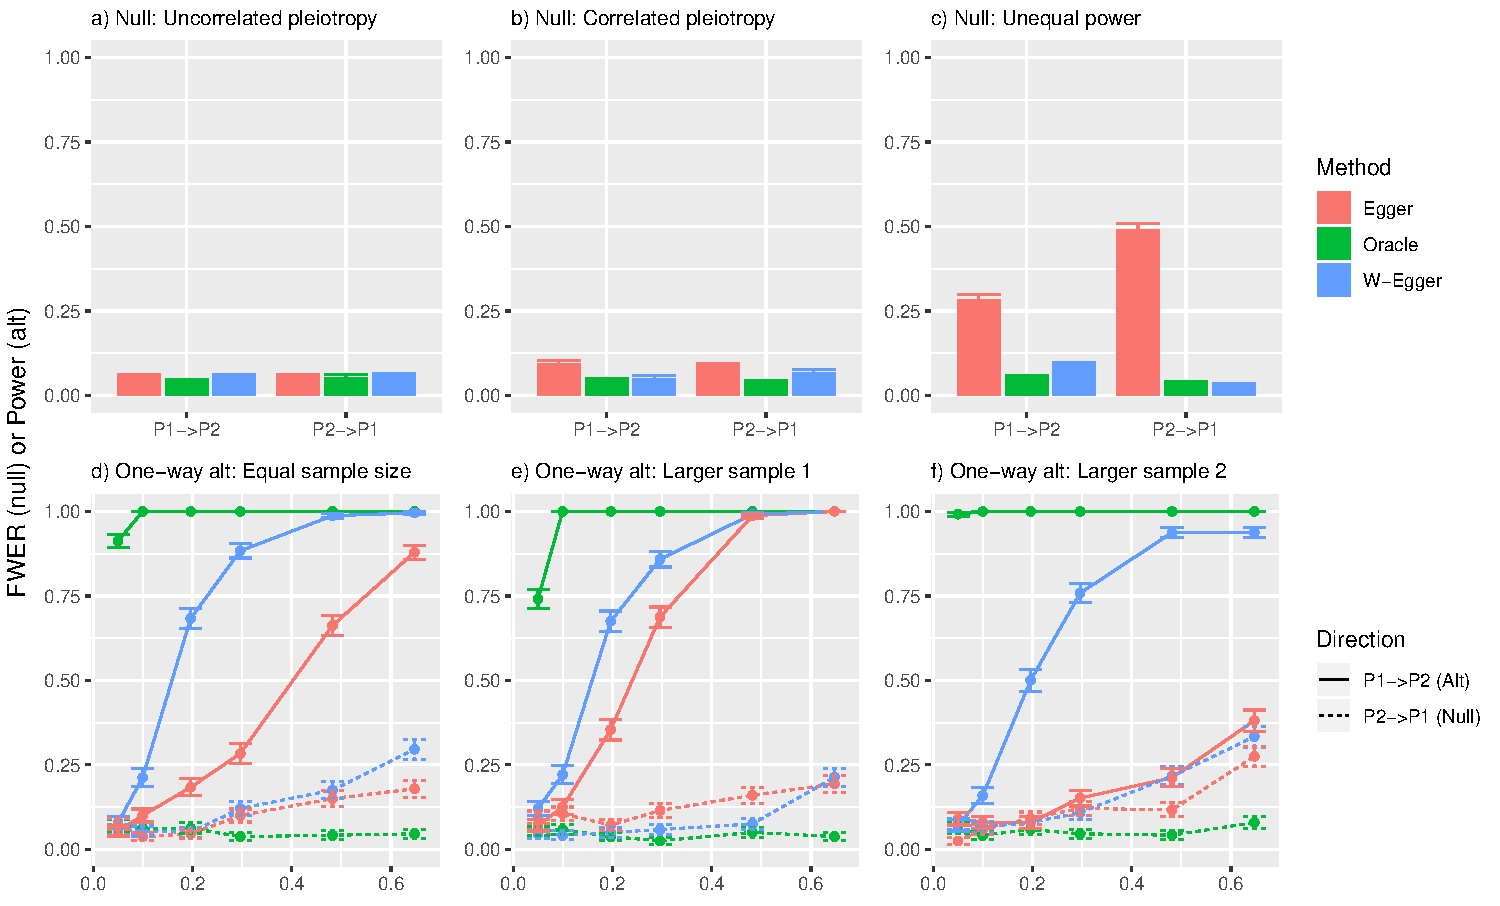
\includegraphics[width=\textwidth]{figures/figure1.pdf}
\caption{Weighted Egger regression reduces false positives and increases power
 in bi-directional MR. We simulated GWAS summary statistics for two phenotypes
  ($A$, $B$) with $M=1,000,000$
independent SNPs, $20\%$ heritability and $N = 100,000$ individuals in both
 the SNP discovery and effect estimation cohorts. In each simulation, there
 were $5,000$ causal SNPs per phenotype. a) Both the effect of A on B and B on A are null,
 and $1000$ of the SNPs have uncorrelated pleiotropic effects. All methods are well behaved.
 b) Both effects are again null, but the $1000$ shared SNPs have equal effects on both
 phenotypes. Egger regression results in excess false positives which our weighting scheme
 reduces. c) Both effects are null and the shared SNPs have an equal effect on both phenotypes,
 but the shared SNPs have twice as large an effect on $B$, which also has a much smaller sample
 size. Egger regression results in numerous false positives, which our weighting scheme corrects.
 d) $A$ has a variable effect on $B$ and the studies have equal sample size. Our weighting
 scheme improves power over standard Egger regression. e) $A$ effects $B$, which has a much
 lower sample size. Our weighting scheme improves power, but not as much as in (d). f) $A$
  effects $B$, but $A$ has a much smaller sample size. Our weighting scheme substantially increases
  power. We conduced $1000$ simulations for each null experiment (a-c) and $250$ simulations
  per effect size for each alternative experiment (d-f). }
\end{figure}

Next, we wanted to asses the power of our approach under the one-way alternate
hypothesis for various true effect sizes. We again conduct thee simulations,
calculating the power for effect sizes ranging from $0.05$ to $0.7$.
In the first, the cohorts had equal sample sizes ($N = 100,000$). In the second, the exposure
cohort has larger sample size ($N_1 = 200,000$, $N_2 = 50,000$),
and in the third the outcome cohort has a larger sample size ($N_1 = 50,000$, $N_2 = 200,000$).
In all settings, our weighted Egger approach shows
a substantial gain in power over standard Egger regression. This is especially
notable for smaller effect sizes, and when the outcome GWAS is larger.
In this latter setting, the power of standard Egger regression is only slightly
higher than the FPR for the null hypothesis on the reverse direction,
while our weighted Egger regression has very high power
(Figure~\ref{figure1}d-f, Table~S2). However, both
methods suffer from an increase in false positives in the reverse direction
when the effect size in the forward direction is strong. For more on this
phenomenon, see section~\ref{discussion}.

Finally, we tested the power of our approach under the two-way alternate
hypothesis. We tested pairs of effects ranging from $-0.5$ to $0.5$ in both cohorts.
Here we conduct two simulations: one with equal sample size of $N=100,000$,
and one with unequal sample sizes $N_1 = 200,000$ and $N_2 = 50,000$.
In all settings, our approach improves power
substantially over standard Egger regression (Figure~\ref{figure2}a-d). As with
the one-way alternative, this is particularly apparent when the outcome has a larger
sample size than the exposure (Figure~\ref{figure2}d). We also observed that both
methods had lower power when $R_{12} \approx -R_{21}$ and vice versa, especially when
$R_{12}$ has large absolute value. Indeed, as $R_{12} \rightarrow -R_{21} \rightarrow 1$, the model
becomes unidentifiable. This setting is actually a violation of the \emph{faithfulness}
assumption commonly employed in causal inference~\cite{Pearl2000}.

\begin{figure}\label{figure2}
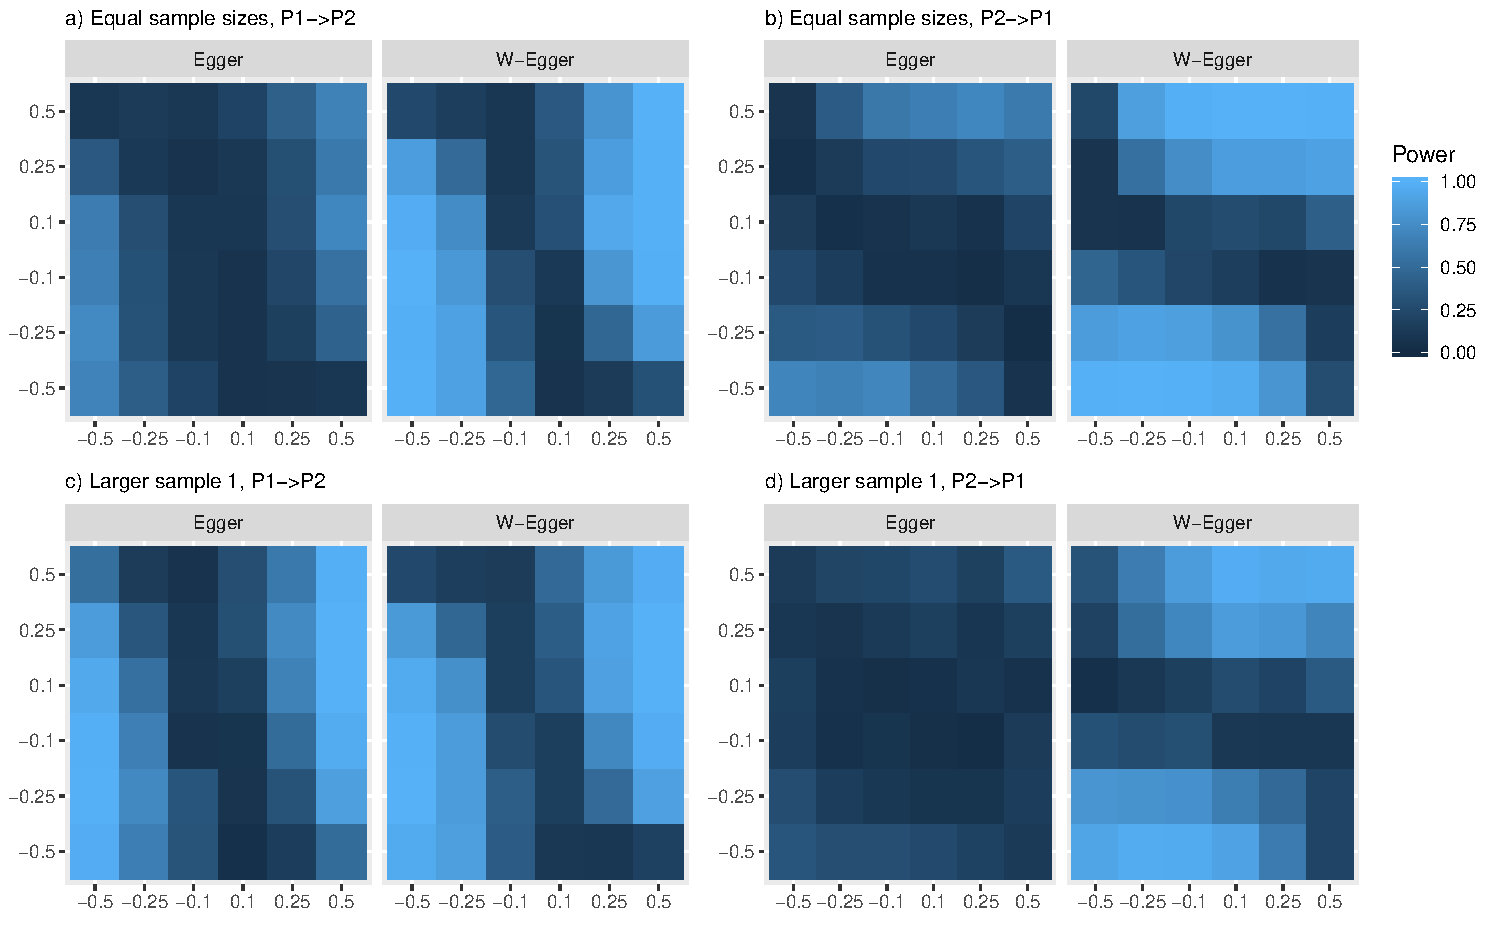
\includegraphics[width=\textwidth]{figures/figure2.pdf}
\caption{Weighted Egger regression improves power under the two-way alt.
 We simulated GWAS summary statistics for two phenotypes ($A$, $B$) with $M=1,000,000$
independent SNPs, $20\%$ heritability and $N = 100,000$ individuals in both
 the SNP discovery and effect estimation cohorts. In each simulation, there
 were $5,000$ causal SNPs per phenotype of which $1,000$ were shared with uncorrelated
 effect sizes. a) Power to detect the effect of $A$ on $B$ when the studies have equal
 sample sizes. Our weighting scheme increases power of standard Egger regression, but both
 methods struggle to detect when the traits cancel each other out. b) Power to detect the
 effect of $B$ on $A$. Our approach improves power and the cancellation pattern is transposed.
 c) Power to detect the effect of $A$ on $B$ when $A$ has a larger sample size. Our approach
 improves power, though both do well. d) Power to detect the effect of $B$ on $A$ when
  $A$ has a larger sample size. Our approach improves power substantially over standard
  Egger regression, which struggles to detect the effect. Results are the average of 250
  simulations per pair of effects.}
\end{figure}

In these simulations, we used a $p$-value threshold of $5\times 10^{-6}$
for all weighted Egger regression analyses, but the conclusions held across a range
from $5\times 10^{-4}$ to $5\times 10^{-8}$. We found that
$5\times 10^{-6}$ provided a reasonable balance between increased power under 
the alternative and control of type-I errors. However, lower
cutoffs will provide better control of the type-I error rate in difficult situations
at the expense of reduced power. Likewise, higher cut-offs yield higher power
while reducing control of the type-I error rate
(Table~S3 and Table~S4). 

\subsubsection*{inspre is competitive with glasso while handling missingness and directed graphs}
As detailed above, both inspre and glasso can be viewed as methods
for finding a sparse, approximate inverse to a noisily measured matrix.
Therefore, we sought to compare these two methods when data are simulated
from the glasso model. We generated data
from a multivariate-normal distribution with a sparse precision matrix
for various graph structures, sample sizes, and numbers of features.
We considered three kinds of graph structures: 1) Erd\"os-R\'eyni (random) graphs,
where each edge is included with probability $p$, 2) hub graphs, where nodes
are partitioned into
disjoint sets and every node in each set is connected to a central ``hub" vertex,
3) scale-free graphs, where the vertex degree distribution
follows a power law. Hub and scale-free networks are intended to mimic common
biological networks~\cite{Barabasi1999}. In each setting we calculated the precision,
the number of true edges among all inferred edges, and recall, the proportion
of true edges detected. We used these to calculate the $F_1$ score, the
harmonic mean of precision and recall, as a function of the
stability of the inferred graph. For the graphical lasso, we used StARS to
evaluate graph stability. For inspre, we used random masks in the weight matrix
as detailed above.

First, we simulated data with $40$ features and $800$ samples. Our random
graphs included each edge with probability $p=0.04$, and our hub graphs had
two hubs of $20$ features each. In this setting inspre and glasso performed
similarly for all graph types, with glasso performing slightly better on
random graphs, inspre performing slightly better on hub graphs, and 
both methods having very similar performance for scale-free graphs
(Figure~S1a-c). Next, we simulated  data with $100$
features and $500$ samples. Here our random graphs included each edge with
probability $p=0.02$ and our hub graphs had $5$ hubs. In this setting, glasso outperformed inspre on
random graphs, inspre outperformed glasso on hub graphs, and both methods again
had similar performance on scale-free graphs, with a slight edge towards
glasso (Figure~S1d-f).

We hypothesized that if the entries in the correlation matrix had variable
sample sizes, the ability of inspre to incorporate weights would improve
performance relative to glasso. This represents a common real-world setting in
which some features are measured on many samples, and some are measured
on only a few. In each simulation, we first chose a maximum missingness
threshold $m$ uniformly between $50\%$ and $99\%$. Then we simulated data with
$100$ features and $2000$ samples. For each feature, we chose
a number between $0$ and $m$ uniformly at random and set that proportion of the features
samples as missing. We then calculated the sample correlation matrix using only
samples where both features were measured per pair of features.
In this setting, inspre was able to continue producing accurate
results even with when the maximum missingness was high. On the other
hand, glasso was not able to produce results at all when there was high
missingness. Instead, the glasso algorithm diverged and the program returned
a matrix of NA values (Figure~S2).


\subsubsection*{bimmer robustly recovers causal direct effect networks}

Our final goal was to show that bi-directional Mendelian randomization
could be combined with inspre to fit networks of simulated phenotypes
from phenome-scale GWAS summary statistics. At the time of this writing
we are not aware of any other methods for this specific problem. However,
there are a few approaches to related problems that could be applied.
Specifically, the CDEs between multiple exposures and a single outcome
can be calculated from a multiple regression of SNP effects on the outcome
against SNP effects on the exposures~\cite{Burgess2015a}. This approach can be used
to find sparse effects by using a LASSO or elastic net regression (elnet-Egger). A more
sophisticated approach, such as MR-Bayesian model averaging (MR-BMA), could also be
applied~\cite{Zuber2020}.
\todo{I would reverse the last two sentences and introduce elnet-Egger as an approximation to MR-BMA.
brielin: I don't think that flows very well.}

First, we simulated summary
statistics for $50$ phenotypes with $1,000$ shared and $2,000$ private
causal effect SNPs per pair of phenotypes, $125,000$ total SNPs. Each
phenotype had $20\%$ heritability. The causal
network underlying the phenotypes came from an Erd\"os-R\'eyni random graph with
randomly oriented edges. We found that MR-BMA performed comparably to
elnet-Egger, but that they both performed poorly compared to bimmer.
Moreover, MR-BMA took about $20$ times longer than bimmer to run with
default parameter settings (Figure~S3).

Next, we performed larger-scale simulations with $100$ phenotypes and
$250,000$ total SNPs. We again
simulated data from Erd\"os-R\'eyni, hub, and scale-free networks. In this setting
both the graph structure and the orientation of the graphs edges are important
variables to consider. The edge orientation will not necessarily be random:
for example, master regulators would have very high out-degree but low in-degree~\cite{Liu2010}.
For all graph types, we tested three ways of orienting the edges in the graph:
 1) randomly set the orientation
of each edge (random), 2) preferentially orient edges towards high-degree nodes (towards),
 and 3) preferentially orient edges away from high-degree nodes (away). See
 Figure~\ref{figure4}a-c for examples of different kinds of graphs with
 different edge orientations. We excluded
MR-BMA from these simulations due to runtime concerns.

We found that bimmer was able to accurately re-construct all graph types and edge
orientations considered, while
elnet-Egger consistently had poor performance (Figure~\ref{figure4}d-i, Figure~S4).
 For Erdos-Reyni graphs, we found that edge orientation did not have an effect on the
 performance of bimmer. This is possibly because the node degree distribution
 doesn't have enough variance to have nodes that consistently pull edges towards
 or away from them in the latter scenarios. For scale-free and hub graphs, we
 found that bimmer performed better when high-degree nodes had edges oriented
 away from them (Figure~\ref{figureS3}). This is particularly interesting as
 it corresponds to the most likely real-world scenario~\cite{Barabasi1999}. Indeed, bimmer
 performed worst in the least realistic scenario: hub graphs with edges oriented
 towards the hubs (Figure~\ref{figure4}e). However even in this challenging setting, bimmer
 is able to accurately infer the causal graph.

\begin{figure}\label{figure4}
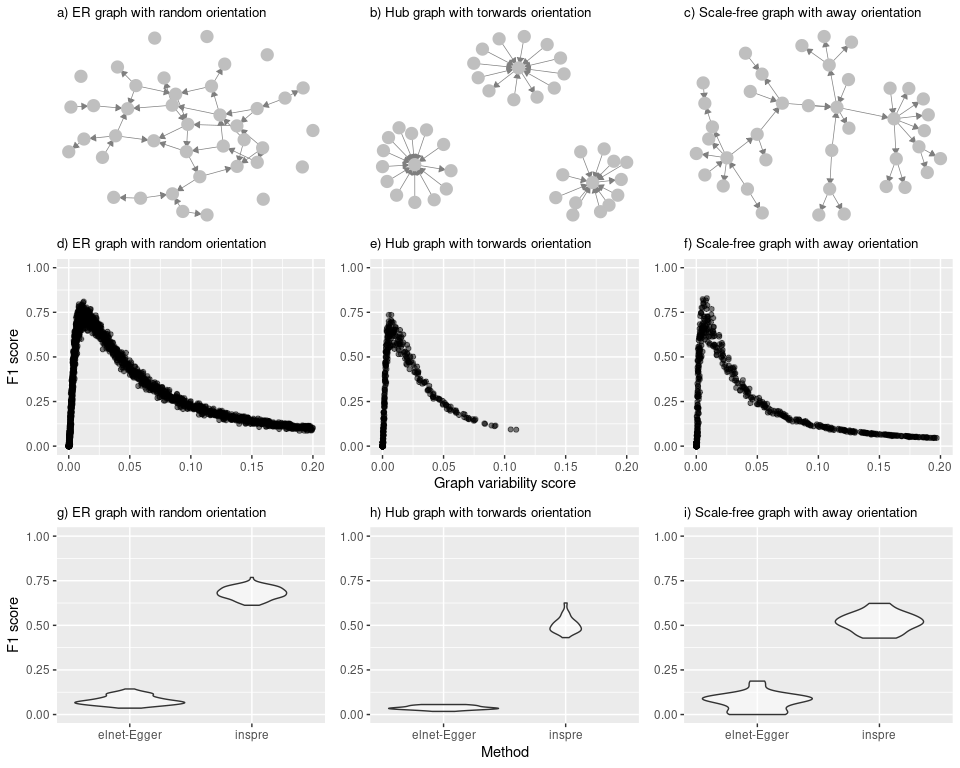
\includegraphics[width=\textwidth]{figures/figure4.png}
\caption{bimmer accurately infers the causal graph for many graph structures and node
orientations. We simulated summary statistics for $100$ phenotypes with $3000$ causal
effects each, $1000$ of which were shared with uncorrelated effects per pair of phenotypes.
We varied the structure and edge orientation of the causal graph underlying the phenotypes.
a) An Erdos-Reyni random graph with randomly oriented edges. Each edge is
included with probability $p=0.05$ and then randomly assigned an orientation. b) A hub
graph with edges preferentially oriented towards high degree nodes. The nodes are split into
three sets and each node in each set is assigned to a central hub vertex. c) A scale-free
graph with edges preferentially oriented away from high degree nodes. These graphs have
node degrees that follow a power-law distribution. We show the $F_1$-score of the method
against the calculated variability score for d) Erdos-Reyni, e) hub and f) scale-free graphs.
In all cases, we are able to produce accurate results when the variability score is between
about $0.01$ and $0.05$. We also compared the performance against Egger regression
with elastic-net shrinkage at a graph variability score of $0.025$. elnet-Egger
performs quite poorly compared to bimmer.}
\end{figure}


\subsection*{Application to 405 traits from the UK Biobank}
\subsubsection*{bimmer identifies thousands of causal effects in complex pathways}
We obtained summary statistics for gender-split UK Biobank phenotypes from
the Neale lab UK Biobank analysis website~\cite{NealeUKBB}. For ease of interpretability,
we transformed all effect sizes to the per-variance scale. As  recommended,
we used only phenotypes with $Z$-score above $4$ and at least medium confidence
~\cite{BulikSullivan2015,NealeUKBB}. Next we removed one phenotype from every pair with genetic
correlation above $0.9$, leaving us with $423$ phenotypes. We clumped the UKBB
summary statistics to $p=5 \times 10^{-6}$ with $r^2 < 0.05$ and distance $500$ kilobases using
the UKBB European genotypes as a reference panel. We use male summary statistics for SNP selection
and weight estimation, and female summary statistics for TCE estimation. Finally, we removed
phenotypes where at least $50\%$ of the standard errors of the TCE were above $0.5$
as either an exposure or an outcome. This left us with $405$ phenotypes (Table S?).
\todo{Table should exist and have degree columns, etc}
From the $163,620$ pairs of traits considered, $8,268~(\sim 5\%)$ had TCEs that
were significant at FDR $5\%$.
Next, we used inspre to fit the model~\ref{r_cde_main}. We used inverse-variance weights
as previously described with one exception - all entries in the TCE matrix with
an SE below $0.005$ were given the same weights. This is to avoid having a very small
number of well-estimated points dominate the optimization procedure. Based on our simulations,
we chose a target stability of $0.025$ which resulted in regularization 
parameter $\lambda = 0.055$. This gave a graph with $7,949$ non-zeros,
$2,826$ of which were above $0.01$. We used these $2,826$ non-zeros as the edges
in our inferred graph.

A few things are immediately apparent when comparing estimates of the
genetic correlation, weighted Egger estimated TCE, bimmer's
shrunk TCE ($U$) and bimmer's inferred CDE. First, we clustered phenotypes by genetic correlation
to determine if the patterns observed are shared in the TCE estimates.
While there are some similar patterns across the two matrices, the structure in the TCE estimates
is not as well-defined (Figure~S5a-b).
Indeed, we find that while the TCE estimates
and genetic correlation estimates are correlated, that correlation is fairly
weak ($r = 0.270\pm 0.005$). We actually find a slightly lower correlation between
 $U$ and $R^{TCE}$ ($r = 0.238 \pm 0.005$), however, this is by design.
Many of our TCE estimates have high standard error and are consequently
ignored by the optimization procedure. Restricting our analysis to TCE entries with an
SE below $0.05$, for example, the correlation of the TCE with the genetic correlation is smaller
than the correlation of the TCE with $U$ ($r = 0.666 \pm 0.005$ vs $r = 0.949 \pm 0.004$, respectively).
Moreover, our optimization
procedure tends to produce entries of $U$ that are very close to $0$ when the corresponding
entry of the TCE has a large standard error ($\bar{|U|} = 0.0003 \pm 0.0003$ for entries of
the TCE with SE $> 0.05$). We conclude that our optimization procedure produces a conservative
estimate $U \approx R^{TCE}$ that is close on high confidence entries of $R^{TCE}$ and
shrunk strongly towards 0 otherwise.


Most ($303/405$, $\sim 75\%$) phenotypes have out-degree $0$ in our network, that is they have no
downstream causal effects. However, there is a path from every node with non-zero
out-degree to every other node in the network. The vast majority of these connections
are indirect and result in small effect sizes that do not reach
statistical significance as TCEs. Connections in the network with FDR-corrected TCE p-value above
$0.05$ have an average absolute shrunk TCE of $0.0036$ and path length of $2.8$ nodes, while
FDR significant connections have an average shrunk TCE of $0.029$ and path length of $1.98$ nodes
(Figure~\ref{figure6}a-b). Even still, we find that the majority of significant TCEs are from indirect
connections ($3,831$ connections, $63.7\%$).
We also found that the effect explained by the shortest path between two nodes was often only a small
fraction of the total effect. That is, there are often multiple paths between two nodes that add together
to form the TCE (Figure~\ref{figure6}c-d). As expected, this is especially pronounced 
when looking at all connections (Figure~\ref{figure6}c) rather than FDR $5\%$-significant connections
(Figure~\ref{figure6}d), however this conclusion holds in both settings.
Among all connections the median percentage of the effect explained
by the shortest path is $0.35\%$, vs $0.52\%$ for FDR-significant connections. It is also important
to point out that this number is not always less than 1. That is, it is sometimes the case that the
effect of the shortest path is greater than the total effect, indicating that other paths between
the nodes act to cancel out the effect of the shortest path and reduce the total effect.

We found that many indirect effects act through central hub vertices with high degree. For example,
body mass index (BMI, in-degree 29, out-degree 215), leukocyte count (in-degree 16, out-degree 224), and
haemoglobin concentration (in-degree 7, out-degree 122), which we discuss in detail in the next
section. We also found that learning the network structure, rather than simply calculating TCEs
for every pair of phenotypes, allows us to both understand potentially surprising effects, and
also identify seemingly significant effects that lack network support.
For example, we observed a strong effect of ``age first had sexual intercourse'' (AFSI) on a number
of surprising outcomes including knee pain ($U = -0.064$, $p < 3 \times 10^{-7}$),
wheezing in the chest ($U = -0.067$, $p < 1 \times 10^{-16}$) and
lower overall health rating ($U = -0.058$, $p < 4 \times 10^{-9}$). A closer look reveals
that all of these effects are mediated by an effect of AFSI on BMI, which does not survive
correction for multiple testing ($R^{TCE} = -0.20 \pm 0.07$, $U = -0.37$, $p < 0.07$),
but is required by the network to explain observed effects of AFSI on the aforementioned phenotypes.
This may lend additional evidence to recent work showing that BMI-associated loci are involved
in brain pathways linked to reward~\cite{Ndiaye2020}.
On the other hand, we find effects with low TCE $p$-values that are not reflected in
the network structure. For example, we observe a strong TCE of cheese intake on time spent watching television
($R^{TCE} = -0.49 \pm 0.07$, $p <  \times 10^{-9}$).
There is indeed a path between these nodes (again mediated by BMI), but the shrunk TCE corresponding
to this path in the network is only $-0.006$. Similarly, we observe a strong TCE of 
past tobacco smoking on ``ever taken cannabis'' ($R^{TCE} = -0.88 \pm 0.13$, $p < 3 \times 10^{-9}$).
Here the path between these nodes flows through BMI, followed by leukocyte count, for a shrunk TCE of
only $-0.0002$.
 

\begin{figure}\label{figure6}
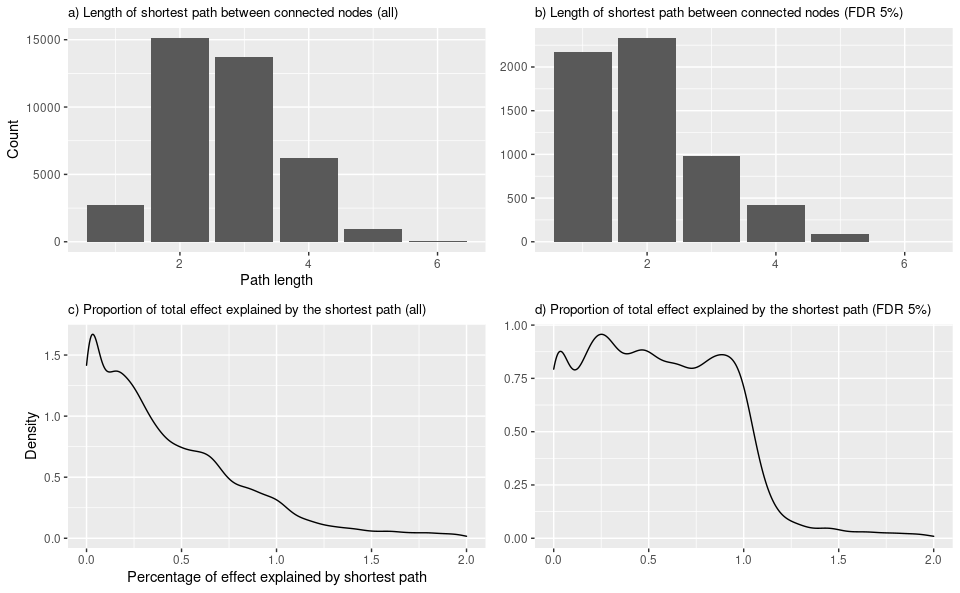
\includegraphics[width=\textwidth]{figures/figure6.png}
\caption{bimmer identifies indirect effects and paths explaining a small proportion of the total effect.
The distribution of path lengths between connected nodes for (a) all connected nodes and (b) connected
nodes with an FDR $5\%$ significant TCE. Our analysis shows that there are many long paths between
nodes that result in very small effect sizes; closer connections are much more likely to reach
significance after correction for multiple testing. Moreover the shortest path often explains only
a fraction of the total effect for both (c) all connected nodes and (d) connected
nodes with an FDR $5\%$ significant TCE, indicating that there are often numerous ways of
getting from one node to another that add together to form the TCE. We also observe that the shortest
path sometimes explains more than the total effect, indicating that other paths between the nodes
act to cancel out the effects of the direct path. }
\end{figure}


\subsubsection*{bimmer identifies concentrated sub-networks with correlated downstream effects}
Our final goal was to identify concentrated sub-networks with correlated downstream effects.
To this end, we clustered phenotypes using their shrunk TCE estimates ($U_{i, :}$) as features.
This results in groups of phenotypes with similar downstream effects being clustered together.
We focused on the $102$ phenotypes with non-zero out-degree.
In Figure~\ref{figure5}, we show the genetic correlation (a), weighted-Egger TCE (b), shrunk TCE (c) and
inferred CDE (d) for these $102$ phenotypes as exposures and all $405$ phenotypes as outcomes. This allows
us to identify several interesting sub-networks with numerous downstream effects. We chose four sub-networks
for futher analysis: a sub-network of morphology-related traits (Figure~\ref{figure5}e),
one of blood-biomarker related traits (Figure~\ref{figure5}f), one of red-blood cell (erythrocyte)
related traits (Figure~\ref{figure5}g), and one of heart-disease related traits (Figure~\ref{figure5}h).
In all cases, every node within the sub-network is reachable from every other node. 
These sub-networks also tend to include traits that are related by definition. In many of these cases,
bimmer puts a bi-directed edge between the two nodes, for example between BMI and weight or
between mean sphered cell volume and mean reticulyte volume. While this does not happen universally,
bimmer generally succeeds at identifying groups of traits which could be analyzed jointly. 

Leukocyte count, part of the heart-disease network, had the highest out-degree with $244$ CDEs
and $177$ FDR $5\%$ significant TCEs. This network includes several well-studied phenomena
including the causal effect of hypertension on heart disease ($p < 3 \times 10^{-5}$~\cite{MacMahon1990}),
and high cholesterol on heart disease ($p < 1 \times 10^{-16}$~\cite{Castelli1992}). We also find
evidence for both a direct causal effect of leukocyte count on heart disease
($p < 2 \times 10^{-3}$~\cite{Lee2001})
and an indirect effects via high cholesterol ($p < 4 \times 10^{-7}$) and diastolic blood pressure
($p < 7 \times 10^{-4}$), both of which are previously studied pathways~\cite{Facchini1992}.
It is also interesting to note that the network places edges between
leukocyte count and both systolic blood pressure and hypertension, but these do not survive correction
for multuple testing as TCEs ($p < 0.055$ and $p < 0.063$, respectively). We consider this evidence of
a complex mechanism by which white blood cell traits effect heart disease risk via multiple causal pathways,
warranting further study. One interesting downstream effect of this sub-network is related
to choice of pain medication. We detect a positive causal effect of high cholesterol on aspirin use
($R = 0.065$, $p < 3 \times 10^{-6}$) and a negative effect on ibuprofen use ($R = -0.025$, $p < 0.001$).
This could reflect common medical advice for patients at risk of heart disease to choose aspirin,
which has long been thought to reduce risk~\cite{Sanmuganathan2001}, and avoid ibuprofen, which
is thought to reduce it's effectiveness~\cite{MacDonald2006}. Another interesting set of traits
downstream of this sub-network are related to personality. We find evidence for a causal effect of
leukocyte count on ``suffer from nerves'' ($p < 1 \times 10^{-10}$), ``worrier / anxious feelings'' 
($p < 2 \times 10^{-10}$), neuroticism score ($p < 1 \times 10^{-7}$) and ``tense / highly strung''
($p < 5 \times 10^{-10}$). This adds to a growing body of literature on a relationship between
inflammatory biomarkers and personality~\cite{Allen2017,Sutin2012}.

The blood biomarker network was particularly dense,
consisting of $255$ direct connections, $236$ of which represent
significant TCEs at FDR $5\%$.
We find that higher testosterone levels have numerous health consequences, many of
which are related to lung function. For example, higher testosterone protects against
shortness of breath ($R = -0.028$, $p < 4\times 10^{-3}$) and asthma ($R = -0.008$, $p < 0.05$)
while increasing risk of lung cancer ($R = 0.013$, $p < 0.02$). This lends causal support to
recent observational studies linking increased testosterone to lung cancer risk~\cite{Hyde2012}
and mouse models linking decreased testosterone to asthma risk~\cite{Cephus2017}.
Our results also support the possibility of a causal effect of sex-hormone
levels on personality~\cite{Colangelo2012,Asselmann2019,Ekholm2014,Aluja2014}.
For example, we observe an effect of testosterone on loud
music exposure frequency ($R = 0.018$, $p < 0.001$), and
an effect of sex-hormone binding globulin on
``been in a confiding relationship as an adult'' ($p < 3 \times 10^{-10}$),
 anxious feelings ($p<4\times 10^{-9}$), neuroticism score ($p<6\times 10^{9}$), and ``suffer from nerves``
($p < 3\times 10^{-7}$). However it is important to point out that these results have been debated. For
example, the findings in~\cite{Asselmann2019} do not survive correction for multiple testing and
in~\cite{Aluja2014} the relationship between sex hormones and personality decreases after controlling
for age. Indeed we generally find that while these effects have very low TCE p-values, they 
are also quite small (bimmer shrunk TCE from $-0.007$ to $0.002$.

BMI has the second-highest out-degree of any phenotype considered with
$215$ direct effects, and $175$ FDR $5\%$ significant TCEs.
Many of the top downstream effects of BMI are dietary
in nature, including vegetable intake ($R = 0.09$, $p < 1\times 10^{-16}$),
milk-type ($R = 0.15$, $p < 1\times 10^{-16}$), and dietary variation ($R = 0.115$, $p < 1\times 10^{-16}$).
This lends additional support to the recent literature on BMI the cause of (and not effect of)
traits thought to lead to higher BMI (ie exercise~\cite{Richmond2014}) and the observation that
BMI-increasing genetic variants tend to be linked to genes with a role in brain
function~\cite{Locke2015,Zhu2016,Ndiaye2020}. Morphology-related traits are also linked
to numerous diseases, perhaps best exemplified by the strong causal effect of BMI on lower overall
health rating ($R = 0.1$, $p < 1 \times 10^{-16}$). It is also interesting to note that the
morphology network includes predicted forced expiratory volume in
one second (FEV-1), a simple function of height, age and ethnicity,
while the erythrocyte network includes measured FEV-1, which is closely related to
erythrocyte function. In the latter network, erythrocyte count and haemoglobin concentration (HC)
both have high out-degree, with $117$ and $132$ direct effects, respectively.
Erythrocyte count has numerous health consequences,
for example a direct effect on lower overall health rating ($R = 0.03$, $p < 3 \times 10^{-10}$).
Many of the top direct effects of HC involve platelet structure,
for example plateletcrit ($R = -0.13$, $p < 3 \times 10^{-11}$) and platelet count
($R = -0.15$, $p < 2 \times 10^{-10}$). Interestingly, our model predicts a direct effect of
HC on bleeding gums ($R = 0.036$, $p < 2 \times 10^{-9}$); that is, one
that is not mediated by the aforementioned effects on platelets. This may reflect a lack of power to detect
the direct effect of platelets on bleeding gums, or indicate that this acts via an alternative pathway.
Finally, we noticed our model predicts a direct effect of HC on cardiac arrythmia, lending causal
support to a recent population-based study linking HC and atrial fibrillation~\cite{Lim2020}.


\begin{figure}\label{figure5}
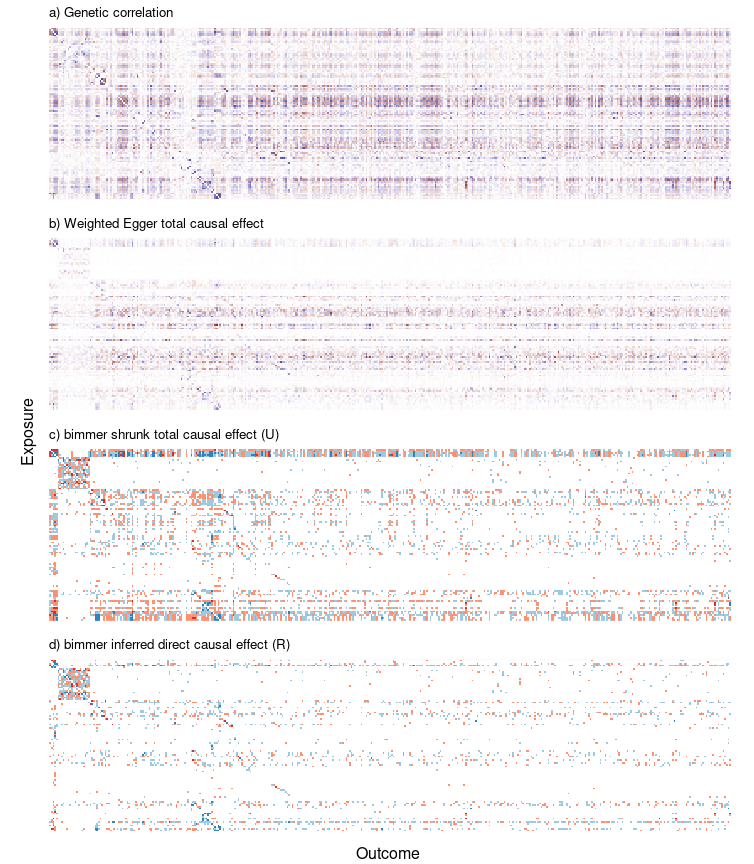
\includegraphics[width=\textwidth]{figures/figure5.png}
\caption{bimmer identifies concentrated sub-networks with correlated downstream effects.
Here we plot (a) the genetic correlation, (b) the weighted Egger TCE, (c) the bimmer shrunk
TCE and (d) the bimmer inferred CDE for the 102 phenotypes with non-zero out-degree (y-axis)
against all 405 phenotypes (x-axis), clustered by shrunk TCE. To emphasize the smaller effects
in the latter plots, we use an alternate scale which emphasizes weak positive and negative effects
(0.01 to 0.1, light blue and red, respectively) and strong positive and negative effects
(0.1 to 1, dark blue and red, respectively). Clustering by shrunk downstream effects reveals
several concentrated sub-networks, including a morphology network (e), blood biomarker
network (f), red blood cell network (g) and heart disease network (f).}
\end{figure}

\section{Discussion}\label{discussion}
As biobanks continue to grow in size and scope, new methods that are able to
leverage their power while overcoming common pitfalls are required.
These datasets offer unprecedented opportunity to study
the causal relationship between molecular markers, complex traits and diseases.
Generally speaking, causal claims should be backed by thorough analysis resulting from
multiple studies with differing assumptions. This raises the question
of whether phenome-scale causal inference, where the number of pairs of to be tested
renders this unrealistic, is even possible. Instead, in this setting researchers should focus on
causal discovery, learning putatively causal structures that can suggest avenues for further
work.
Here, we have introduced bi-directional mediated Mendelian randomization (bimmer),
a novel approach to inferring sparse networks of causal direct effects from phenome-scale
GWAS summary statistics. We have shown through extensive simulations that
bimmer is able to learn many kinds of causal graph structures even in the presence
of non-causal genetic correlation and differential power across phenotypes.
We have demonstrated that our method enables researchers to conduct 
analyses that would otherwise be extremely difficult. For example, 
we are able to interrogate the complexity of the network by analyzing the path length
distribution and proportion of effect explained by the shortest path. We also able to 
interpret surprising TCEs in the context of the network structure, find seemingly
significant TCEs that are not able to be supported by the graph  structure, and
identify concentrated sub-networks that can be analyzed jointly. By applying our
method to the UK Biobank, we lend causal support to several recent observational studies.

While we are not aware of other methods for this problem, our approach
builds on recent MR literature. In particular, multi-variable Mendelian
randomization methods are able to compute causal direct effects when there
are multiple potential exposures and a single outcome~\cite{Zuber2020,Burgess2015a}. While
these methods work well in that setting, we have shown that they are not well-suited
to the more general network inference problem that we consider here. Another approach, network
Mendelian randomization, calculates the effect of an exposure on an outcome while
accounting for the effects of a third variable~\cite{Burgess2015}. Our method can
be thought of as a generalization of this approach to an arbitrary number of phenotypes
without pre-specifying any as exposures or outcomes. The first step in our method
involves bi-directional MR with Egger regression weights that reduce the effect
of pleiotropic SNPs. This is related to several recent methods.
In particular, gwas-pc uses asymmetry in the effect size distributions
to choose an effect direction between the two phenotypes. Similarly, 
LCV uses this asymmetry to fit a latent variable model, where imbalanced
genetic correlation between the phenotypes and latent variable imply
the effect direction. Compared to these methods, our approach offers several
advantages. First, like LCV but unlike gwas-pc, our method controls the type-I error rate
when there is non-causal genetic correlation and differential power. Second, like gwas-pc,
but unlike LCV, our method estimates a quantity that is interpretable as the
effect of one phenotype on the other. Finally unlike both,
we are able to estimate both effect directions simultaneously, allowing our
model to accommodate graphs with cycles. In principle, bimmer can use any MR method
that is able to produce bi-drected effect estimates in-place of weighted Egger
regression, allowing researchers to choose the method that best accommodates the assumptions of
the setting they work in.

However, our approach also has several disadvantages. First, our method
requires that we split the initial cohort into instrument discovery and
effect estimation sub-cohorts. This is common in MR methods, but LCV has
the distinct advantage of using all SNPs, which obviates the need
for sample splitting and should improve power. Second, while there are some
phenotype pairs where a direct cause makes sense, there are others where causality is 
almost certainly better interpreted as the action of a latent variable. Indeed, it is likely
that some of the causal effects we infer actually represent shared causal pathways.
Finally, our method suffers from a modest increase in false positives in the $B\rightarrow A$
direction when there is a strong effect from $A\rightarrow B$. When there are many
causal SNPs and the effect of $A$ on $B$ is strong, some SNPs that directly effect $A$
can be mistakenly used as instruments for the effect of $B$ on $A$. While our method
reduces the magnitude of this estimated effect, it can still give some false positives.
Our approach also still suffers from weak instrument bias, generally underestimating
the causal effect, which reduces power~\cite{Davies2015}.

The second step of our method involves finding a sparse inverse to a noisily measured
matrix, and is therefore closely related to the graphical lasso. Like glasso, our method
 has a single regularization parameter that can be set in a straightforward manner.
However, a key advantage of our approach is that we are able to incorporate
weights. This is extremely important in our application since the standard errors
of the TCE matrix can vary dramatically. This also allows us to approximately invert matrices
with missing data, implicitly performing matrix completion by leveraging assumed
sparsity in the inverse of the matrix. Another advantage
of this approach is that it allows us to select the lasso parameter $\lambda$ without
access to the underlying data by using random masks.
A final advantage is that this step in our approach makes no
assumptions about the data generating process, unlike glasso which assumes the data are
multivariate normal. We found that for many classes of graphs,
inspre and glasso produced similar results, however there were some settings where glasso
clearly performed better and vice versa.
Moreover, our method is substantially slower than glasso, with
complexity $O(??)$ compared to glassos $O(??)$. In spite of these limitations,
we believe the advantages of our method for graph inference mean that it will find utility
outside the scope of MR.

Another advantage of our approach is that it only requires GWAS summary statistics.
While the UK BioBank primary genotypes and phenotypes are readily available, summary
statistics are much easier to share and faster to work with when the primary
data is large~\cite{Pasaniuc2017}. They also enable researchers to work with data from a
standardized analysis pipeline~\cite{NealeUKBB}.
Strictly speaking, our method does not even require summary statistics. If
MR analysis results are already available for every pair of a set of phenotypes,
one can use them to construct the matrix $R^{TCE}$ and then infer $R$ with
bimmer. In this setting, it is of paramount importance that the researcher verify
the underlying studies were conducted in a way to minimize the effect of
horizontal pleiotropy.


In this work we have begun to elucidate the connection between Mendelian randomization
and the omnigenic model~\cite{Boyle2017}. The effects of genetic variants
can be used to find and orient edges
in the causal graph underlying the phenotypes, and long-range effects can be modeled
as paths in this sparse graph resulting in ubiquitous but small effects.
 Our method can be applied well beyond the scope considered
here. We are particularly interested in the application to datasets of molecular phenotypes.
These datasets generally have much smaller sample sizes, but molecular phenotypes also
tend to be less polygenic with larger, localized SNP effect sizes, which improves the efficiency
of MR. Inverse sparse regression could also be applied to datasets from CRISPR-based
genetic perturbation experiments, where it could improve the accuracy of network estimation.
We view all of these applications as important avenues for future work.

\section{Methods}\label{methods}
\subsection{Trait model}
As detailed above, our goal is to estimate a sparse causal graph, $R$, from
summary association statistics between genotypes $X$ and phenotypes $Y$. We model
the SNP effects $\beta$ and the causal graph as fixed, and assume that the genotypes
$X$ are sampled uniformly from a population. For convenience, we assume that SNPs
 and phenotypes have been normalized
 to have mean $0$ and variance $1$. We also assume that SNPs are uncorrelated (no LD)
and use LD-pruned variants in all analyses of real data.
Consider fitting the above model $Y = (X\beta + \gamma)(I-R)^{-1} + \epsilon$
using two-stage least-squares with $X$ as instruments. For now,
 assume each SNP acts only on one phenotype
(there is no pleiotropy) and that we know which phenotype it is.
First regress each instrument on it's phenotype and use these effect
 estimates to calculate a set of phenotype scores for each individual.
Next, regress each phenotype score on the observed values of the other phenotypes,
 creating a matrix containing estimates of the total causal effect (TCE) of
 each phenotype on every other. This gives observed effect matrix $\hat{\beta}$,
\begin{align*}
\hat{\beta}_{ij} &= \left\{
 \begin{array}{ll}
  \frac{1}{N} X_{:, i}^{\top}Y_{:,j} & |\beta_{i,j}| > 0 \\
  0 & otherwise
 \end{array} \right. \\
 \mathbb{E}[\hat{\beta} ] &= \beta (I-R)^{-1} \circ \mathds{1}[|\beta| > 0]
\end{align*}
where $\mathds{1}$ is an indicator function and $\circ$ is the Hadamard matrix
product. The TCE matrix is then given by

\begin{align*}
\hat{R}^{TCE} &= \frac{1}{N} (X\hat{\beta})^{\top} Y \\
  &= \frac{1}{N} (X\hat{\beta})^{\top} Y R + \frac{1}{N}(X\hat{\beta})^{\top} X \beta +
     \frac{1}{N}(X\hat{\beta})^{\top} \gamma + \frac{1}{N}(X\hat{\beta})^{\top} \epsilon \\
\mathbb{E}[\hat{R}^{TCE}]  &= \mathbb{E}[\hat{R}^{TCE}] R + D[\beta (I-R)^{-1}]
\end{align*}
where the diagonal operator $D[X]_{i,j} = \left\{ \begin{array}{ll}
  X_{i,j} & i=j \\ 0 & i \neq j \end{array} \right.$ sets off-diagonal elements
  of a matrix to 0.
  Since $\mathbb{E}[\hat{R}^{TCE}] =R^{TCE}$,
this tells us that $R^{TCE}$ satisfies the recurrence
  $R^{TCE}$ = $R^{TCE} R$ off the diagonal, from
  which it follows that~\cite{Pachter},
\begin{equation}\label{r_cde}
R = I - R^{TCE^{-1}} D[1 / R^{TCE^{-1}}]
\end{equation}
where $/$ indicates elementwise division.

In practice we don't know which SNP effects which phenotype,
and there can be correlated pleiotropic effects.
Intuitively, non-pleitropic SNPs will obey the relationship
\begin{equation}\label{MR}
\beta_{k,j} \approx \beta_{k,i} R_{i,j}
\end{equation}
thereby contributing
$\beta_{k, i}^2 R_{i, j}^2$ to the variance of $Y_j$, whereas
pleiotropic SNPs will contribute $\beta_{k, i}^2 R_{i, j}^2 + \alpha^2$
for some pleiotropic effect size $\alpha$. Therefore, SNPs that appear to
have a larger absolute effect on the exposure relative to the outcome in a discovery 
cohort are more likely to satisfy~\eqref{MR}.
 First, we split the samples
 into discovery and estimation sets, generating
two sets of summary statistics $\hat{\beta}_{dis}, \hat{s}_{dis}$ and
$\hat{\beta}_{est}, \hat{s}_{est}$. Next, for each
phenotype $i$ we identify the set of SNPs marginally associated at p-value threshold $p$.
Call this set $I_i = \{k: \hat{p}_{k, i} < p\}$. For every SNP $k \in I_i$ and
every phenotype $j$, we calculate the  weight for SNP $k$ in the regression of $j$ on $i$ as
$w^{i,j}_k = \frac{|\hat{\beta}_{k, i}| - |\hat{\beta}_{k, j}|}
  {\sqrt{\hat{s}_{k,j}^2 (\hat{s}^2_{k, i} + \hat{s}^2_{k, j})}}$. This
  is based on the Welch test for a two-sample difference in mean~\cite{Welch1947}.
  
\subsection{Inverse sparse regression}
If we knew $R^{TCE}$ exactly, we could simply invert it and plug the inverse
into~\eqref{r_cde}. However, our estimate $\hat{R}^{TCE}$ is not necessarily
well-conditioned or even invertable. Instead observe that in ~\eqref{r_cde}, $R$ is
sparse if and only if $\hat{R}^{TCE^{-1}}$ is sparse, and so we can think of
solving~\eqref{r_cde} as finding a sparse matrix inverse. Let $A$ be an arbitrary $D\times D$
matrix. We seek matrices $U$, $V$ with $VU=I$ that minimize the loss,

\begin{equation}
\frac{1}{2} ||W \circ (A - U)||_F^2 + \lambda \sum_{i\neq j}|V_{ij}|
\end{equation}

We minimize this loss using alternating direction method of multipliers (ADMM)~\cite{Boyd2010}.
Let $\Theta^k$ be a matrix of Lagrange multipliers. The updates for $U^k$, $V^k$ and $\Theta^k$
are
\begin{align}
V^{k+1} &\leftarrow \arg \min_{V} \left|\left|\frac{1}{\sqrt{\rho}}\left(I-\theta^{k^\top}\right) -
      \sqrt{\rho} U^{k^\top} V^k\right|\right|_F^2 + \lambda \sum_{i\neq j} \left|V^k_{ij} \right| \\
U_{:, d}^{k+1} &\leftarrow \left(\rho V^{k+1 ^ \top} V^{k+1} + D[W_{:, d}]\right)^{-1} \left(\rho V^{k+1 ^ \top}_{:, d} -
  \left(V^{k+1 ^ \top} \theta\right)_{:, d} + (W \circ A)_{:, d}\right) \\
\theta^{k+1} &\leftarrow \theta_{k} + \rho(V_{k+1}U_{k+1}-I)
\end{align}
where $\rho$ is the penalty parameter~\cite{Boyd2010}.
The first of these can be solved with a straightforward LASSO regression. For the second,
we use the bigconjugate gradient stabilized method implemented
in the Rlinsolve package to solve the linear system
rather than explicitly computing the inverse~\cite{You2018}.
We always start from the initial condition $U_0 = V_0 = I$.
 For the derivation of these equations including
the specifics of how we set
the penalty parameter see the Supplemental note.

\subsection{Setting the LASSO penalty}
Let $\phi_{\lambda}$ be a $D\times D$ matrix where entry $i, j$ is the probability that each edge
$i,j$ is included in the graph for regularization setting $\lambda$. Our goal is to
estimate $\phi_{\lambda}$ for many choices of $\lambda$ and
turn this into a graph instability measure $D_\lambda$.
Let $W^k_{i,j} = W_{i,j}$ with probability $p$ and $W^k_{i,j} = 0$ with
probability $1-p$. Let $V_{\lambda}^k = f(A, W^k, \lambda)$ be
 the function approximating the inverse of
$A$ for regularization setting
$\lambda$ and weight set $W^k$. Let $\psi^k_{\lambda} = \mathds{1}[V^k_{\lambda} > 0]$.
Then  $\phi_{\lambda}$ can be estimated as
\begin{equation}
\hat{\phi}_{\lambda} = \frac{1}{K} \sum_{k=1}^K \psi^{k}_{\lambda}
\end{equation}
using $K$ independent random masks.
The instability measure $D_\lambda$ is estimated as~\cite{Liu2010}
\begin{equation}
\hat{D}_\lambda = \frac{1}{D(D-1)} \sum_{i, j} 2 \hat{\phi}^{i, j}_\lambda(1-\hat{\phi}^{i, j}_\lambda)
\end{equation}

Clearly, $D = 0$ for very large values of $\lambda$, where $V^k_\lambda = I$
for every mask $k$. As $\lambda$ becomes smaller, $D$ rises, but as lambda approaches $0$,
$D\rightarrow 0$ as $V^k_\lambda \rightarrow A^+$. Following~\cite{Liu2010},
we first normalize $\hat{D}_\lambda$ by setting it to
$\bar{D}_\lambda = \sup_{l \leq \lambda} \hat{D}_l$ and then choose the smallest
value of lambda with stability below a cut point $b$,
$\hat{\lambda} = \sup \{ \lambda : \bar{D}_\lambda \leq b \}$.


\printbibliography

\beginsupplement
\section*{Supplemental Note}
\subsection*{Alternating direction method of multipliers}\label{note}
First, consider the unweighted optimization problem
\begin{equation}
\frac{1}{2} ||A - U||_F^2 + \lambda \sum_{i\neq j}|V_{ij}|
\end{equation}
The augmented Lagrangian is,
\begin{equation*}
L = \frac{1}{2} ||A - U||_F^2 +
   \lambda \sum_{i\neq j}|V_{ij}| +
   \Tr(\theta(VU-I)) + 
   \frac{1}{2} \rho ||VU-I||_F^2
\end{equation*}
The update for $V$ can be found by noticing that minimizing $L$ is equivalent
to solving a lasso regression with design matrix $\sqrt{\rho} U^\top$ and
response $\frac{1}{\sqrt{\rho}}(I-\theta^\top)$,
\begin{align*}
   L \propto& \Tr(\theta(VU-I)) + 
     \frac{1}{2} \rho ||VU-I||_F^2 + \lambda \sum_{i\neq j}|V_{ij}| \\
   &= ||\frac{1}{\sqrt{\rho}}(I-\theta^\top) -
      \sqrt{\rho} U^\top V||_F^2 + \lambda \sum_{i\neq j}|V_{ij}|
\end{align*}
The update for $U$ can be found by taking the gradient $\triangledown_U L$
and setting it to 0,
\begin{align*}
\triangledown_U L &= A - U + V^\top \theta + \rho V^\top(VU-I) \\
U &= (I + \rho V^{\top} V)^{-1}(A + \rho V^\top - V^\top \theta)
\end{align*}
ADMM gives the update for $\theta$~\cite{Boyd2010},
\begin{equation}
\theta \leftarrow \theta + \rho(VU-I)
\end{equation}

Now we consider the weighted version. Assume that in addition to the matrix $A$, we
also have a matrix of standard errors of the entries of $A$, $S_A$. Let
$W = 1/S_A^2$ be a matrix of inverse variance weights. We now
seek matrices $U$, $V$ with $VU=I$ that minimize the loss,

\begin{equation}\label{opt_weights}
\frac{1}{2} || W \circ (A - U)||_F^2 + \lambda \sum_{i\neq j}|V_{ij}|
\end{equation}
This does not effect the update for $V$, however the gradient of the augmented
Lagrangian with respect to $U$ is now,
\begin{equation*}
\triangledown_U L = - W \circ (A- U) + V^\top \theta + \rho V^\top V U - \rho V^\top
\end{equation*}
which separates over columns of $U$, giving the update
\begin{equation}
U_{:, d} = (\rho V^\top V + D[W_{:, d}])^{-1}(\rho V^\top_{:, d} -
  (V^\top \theta)_{:, d} + (W \circ A)_{:, d})
\end{equation}
where here the $D$ operator creates a matrix with $W_{:, d}$ on the
diagonal and 0 elsewhere.


ADMM also requires that we set the parameter $\rho$, which controls the
balance in the objective between the primal and dual constraints~\cite{Boyd2010}. We
follow standard practice of setting rho to an initial value and increasing
or decreasing it according to the ratio of the solution to the primal
and dual feasibility constraints. The primal residual at iteration $k+1$ is
given by $r^{k+1} = V^{k+1} U^{k+1} - I$. The dual residual is found by
setting $\triangledown_{U} L^k = 0$ and evaluating it at $U_{k+1}$
\begin{align*}
\triangledown_U L^{k} &= A - U^{k+1} + V^{k^\top} \theta^k + \rho V^{k^\top}(V^k U^{k+1}-I) \\
  &= A - U^{k+1} + V^{k^\top} \theta^k + \rho V^{k^\top}r^{k+1} + \rho V^{k^\top}(V^k U^{k+1}-V^{k+1} U^{k+1}) \\
  &= A - U^{k+1} + V^{k+1^\top} \theta^{k+1} + \rho V^{k^\top}(V^k - V^{k+1})U^{k+1}
\end{align*}
Therefore the dual residual is~\cite{Boyd2010}
\begin{equation*}
d_k = \rho V^{k^\top}(V^k - V^{k+1})U^{k+1}
\end{equation*}
and we can adjust $\rho$ as follows,
\begin{equation*}
\rho^{k+1} = \left\{ \begin{array}{ll}
  \tau \rho^k & if\quad ||r^k||_2 > \mu ||d^k||_2 \\
  \rho^k/\tau & if\quad ||d^k||_2 > \mu ||r^k||_2 \\
  \rho^k & otherwise \end{array} \right.
\end{equation*}
which reduces the impact of the initial choice of $\rho$. While this
may appear to be a lot of parameters, they effect the convergence of
the algorithm substantially more than the solution obtained.
We always use the default values $\rho = 10,\;\mu = 10,\;\tau = 2$.

\newpage
\begin{figure}[H]\label{figureS1}
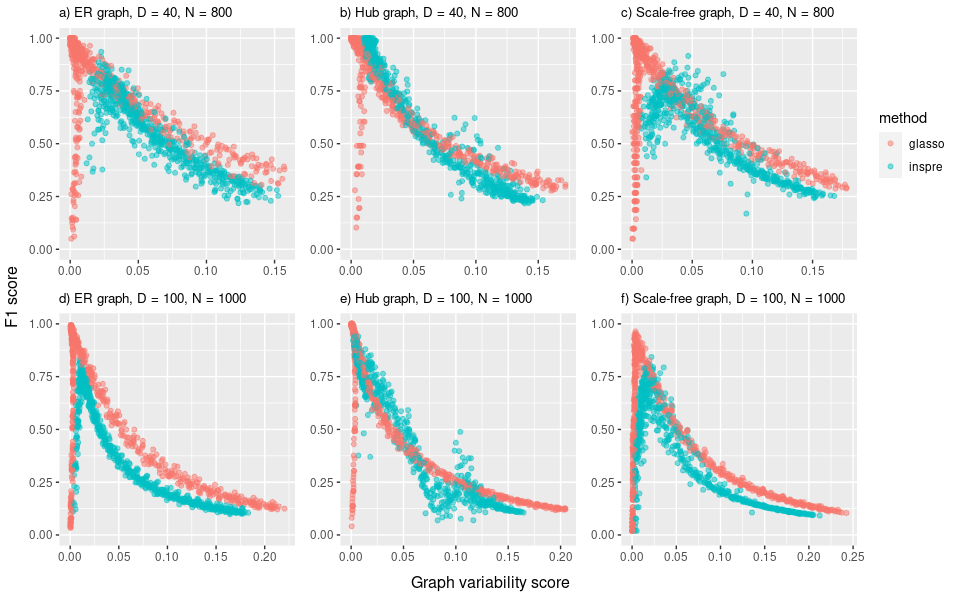
\includegraphics[width=\textwidth]{figures/figure_S1.png}
\caption{inspre performs similarly to glasso on data from gaussian graphical models.
We simulated data from a multivariate normal distribution with a sparse precision matrix
for various sample sizes, dimensionalities and graph structures. Then we evaluated the
relationship between $F_1$-score and graph stability for both inspre and glasso. a) inspre
and glasso perform similarly for Erdos-Reyni graphs, b) hub graphs and c) scale-free graphs
with 40 dimensions and 800 samples. d) At 100 features and 500 samples,
glasso outperforms inspre on Erdos-Reyni graphs,
but the opposite is true for hub graphs (e). f)
glasso also slightly outperforms inspre on scale-free graphs in this setting.}
\end{figure}

\newpage
\begin{figure}[H]\label{figureS2}
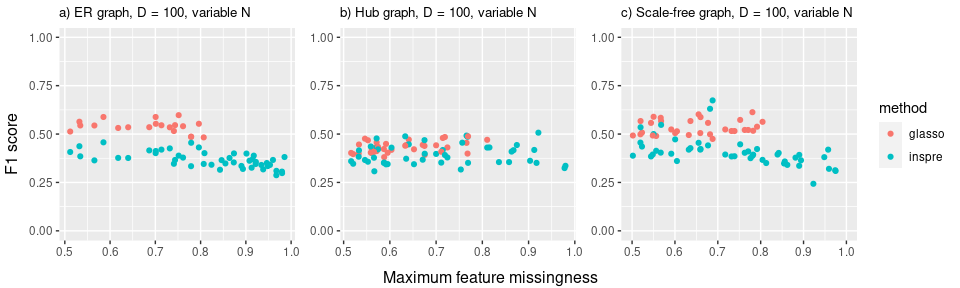
\includegraphics[width=\textwidth]{figures/figure_S2.png}
\caption{inspre is able to produce results when there is differential sample size across
features while glasso diverges. We simulated data from a gaussian graphical model with 100
features and samples sizes ranging from $20-2000$ per feature. inspre continues to produce
results when some features have only $20-400$ samples, while glasso needs at least $400$
for a) Erdos-Reyni, b) hub and c) scale-free graphs.}
\end{figure}

\newpage
\begin{figure}[H]\label{figureS4}
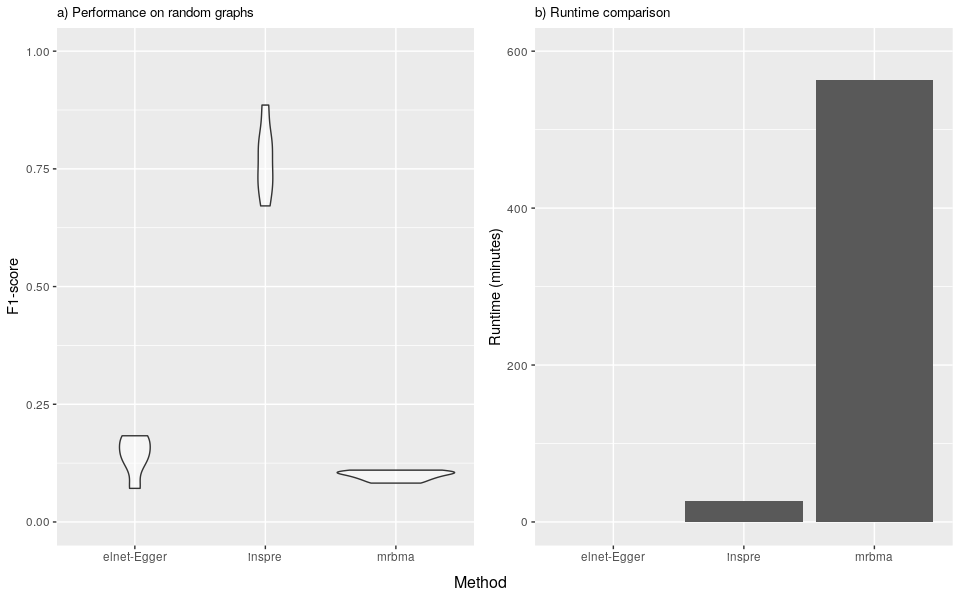
\includegraphics[width=\textwidth]{figures/figure_S4.png}
\caption{bimmer accurately infers small random graphs much faster than MR-BMA. We simulated
Summary statistics for $40$ phenotypes with $3000$ causal
effects each, $1000$ of which were shared with uncorrelated effects per pair of phenotypes.
a) inspre outperforms both elnet-Egger and MR-BMA, which takes about 20 times
longer to run than inspre (b).
}
\end{figure}

\newpage
\begin{figure}[H]\label{figureS3}
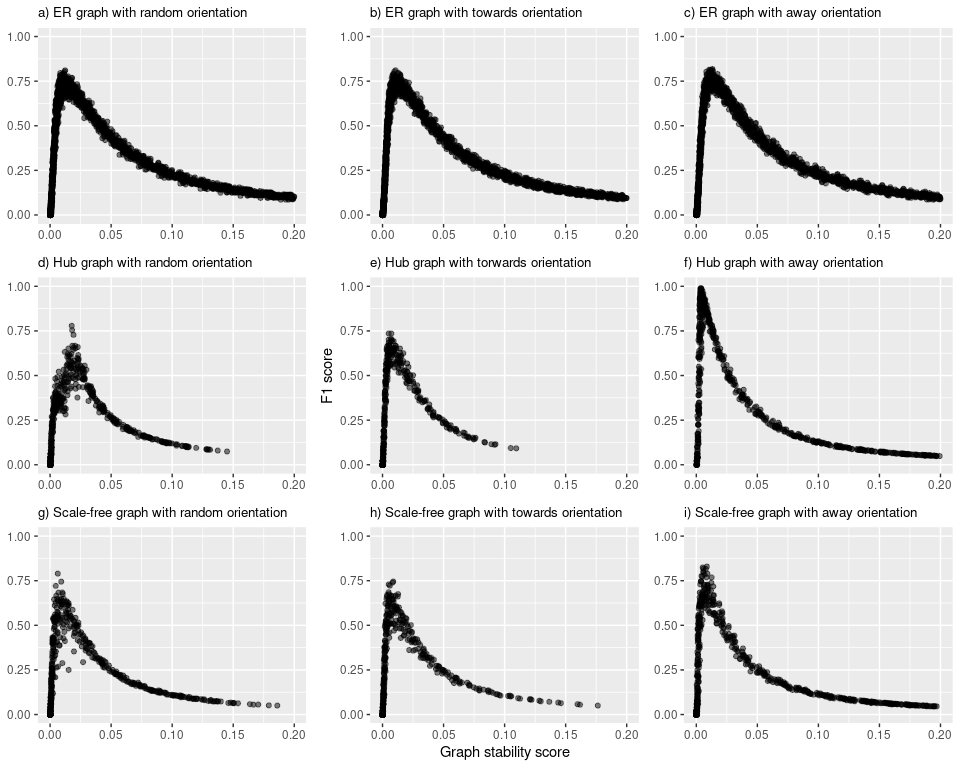
\includegraphics[width=\textwidth]{figures/figure_S3.png}
\caption{bimmer accurately infers the causal graph for many graph structures and node
orientations. We simulated summary statistics for $100$ phenotypes with $3000$ causal
effects each, $1000$ of which were shared with uncorrelated effects per pair of phenotypes.
We varied the structure and edge orientation of the causal graph underlying the phenotypes.
We show the $F_1$-score of the method against the stability score for a) Erdos Reyni graphs
with randomly oriented edges, b) Erdos-Reyni graphs with edges oriented towards high-degree nodes
, c) Erdos-Reyni graphs with edges oriented away from high-degree nodes, d)
hub graphs with randomly oriented edges, e) hub graphs with edges oriented towards high-degree
 nodes, f) hub graphs with edges oriented away from high-degree nodes, g)
scale-free graphs with randomly oriented edges, h) scale-free graphs with edges oriented towards
 high-degree  nodes, i) scale-free graphs with edges oriented away from high-degree nodes. }
\end{figure}

\newpage
\begin{figure}[H]\label{figureS5}
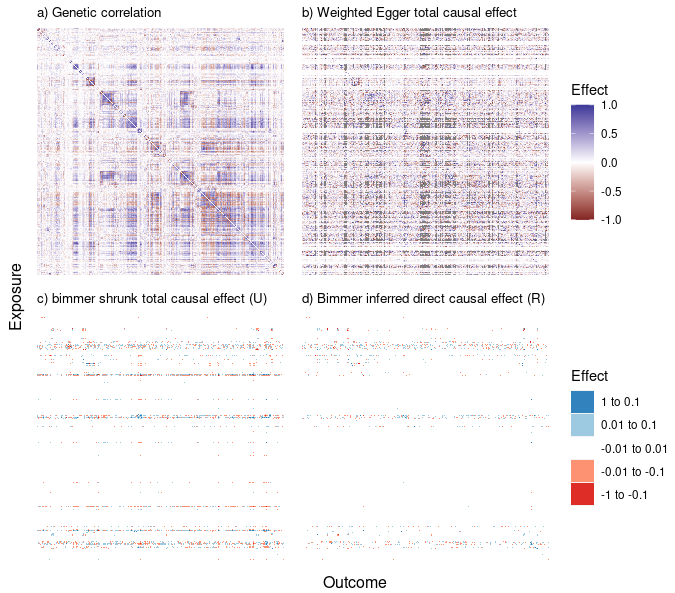
\includegraphics[width=\textwidth]{figures/figure_S5.png}

\caption{bimmer shrunk total causal effects are only weakly correlated with genetic correlation.}
\end{figure}

\newpage
\begin{table}[H]\label{table1}
\centering
\begin{tabular}{lrrrrrrrr}
\toprule
Method & stat1 & se\_stat1 & stat2 & se\_stat2 & mae1 & se\_mae1 & mae2 & se\_mae2\\
\midrule
\addlinespace[0.3em]
\multicolumn{9}{l}{\textbf{Null: Uncorrelated pleiotropy}}\\
\hspace{1em}Oracle & 0.041 & 0.006 & 0.054 & 0.007 & 0.009 & 0.000 & 0.009 & 0.000\\
\hspace{1em}W-Egger & 0.053 & 0.007 & 0.058 & 0.007 & 0.042 & 0.001 & 0.042 & 0.001\\
\hspace{1em}Egger & 0.053 & 0.007 & 0.053 & 0.007 & 0.091 & 0.002 & 0.090 & 0.002\\
\addlinespace[0.3em]
\multicolumn{9}{l}{\textbf{Null: Correlated pleiotropy}}\\
\hspace{1em}Oracle & 0.043 & 0.006 & 0.038 & 0.006 & 0.009 & 0.000 & 0.009 & 0.000\\
\hspace{1em}W-Egger & 0.051 & 0.007 & 0.068 & 0.008 & 0.044 & 0.001 & 0.047 & 0.001\\
\hspace{1em}Egger & 0.095 & 0.009 & 0.084 & 0.009 & 0.172 & 0.004 & 0.166 & 0.004\\
\addlinespace[0.3em]
\multicolumn{9}{l}{\textbf{Null: Correlated pleiotropy, unequal power}}\\
\hspace{1em}Oracle & 0.052 & 0.007 & 0.036 & 0.006 & 0.014 & 0.000 & 0.006 & 0.000\\
\hspace{1em}W-Egger & 0.087 & 0.009 & 0.029 & 0.005 & 0.053 & 0.001 & 0.080 & 0.002\\
\hspace{1em}Egger & 0.284 & 0.014 & 0.492 & 0.016 & 0.178 & 0.003 & 0.648 & 0.010\\
\bottomrule
\end{tabular}
\caption{Weighted Egger regression reduces false positives
 in bi-directional MR under the two way null. We simulated GWAS summary statistics for two
 phenotypes ($A$, $B$) with $M=1,000,000$
independent SNPs, $20\%$ heritability and $N = 100,000$ individuals in both
 the SNP discovery and effect estimation cohorts. In each simulation, there
 were $5,000$ causal SNPs per phenotype and neither phenotype had an effect on the other.
  In the first setting pleiotropic effects are
 uncorrelated and all methods are well behaved. In the next setting the $1000$ shared SNPs
  have equal effects on both phenotypes. Here Egger regression results in excess false positives
  which our weighting scheme reduces. In the last setting shared SNPs again have equal effects
  on both phenotype, but shared SNPs explain a larger proportion of the variance in the
  second cohort, which also has a smaller sample size. Here Egger regression results in numerous
  false positives, which our weighting scheme corrects. Values reflect averages
  over $1,000$ simulations.}
\end{table}
\todo{Merge separate columns into stat (SE) and relabel right before submitting and 1/2->A/B}

\newpage
\begin{table}[H]\label{table2}
\centering
\begin{tabular}{lrrrrrrrr}
\toprule
Method & stat1 & se\_stat1 & stat2 & se\_stat2 & mae1 & se\_mae1 & mae2 & se\_mae2\\
\midrule
\addlinespace[0.3em]
\multicolumn{9}{l}{\textbf{Alt: Equal sample sizes, R=0.2}}\\
\hspace{1em}Oracle & 1.000 & 0.000 & 0.062 & 0.016 & 0.040 & 0.001 & 0.010 & 0.000\\
\hspace{1em}W-Egger & 0.683 & 0.030 & 0.050 & 0.014 & 0.075 & 0.003 & 0.046 & 0.002\\
\hspace{1em}Egger & 0.183 & 0.025 & 0.046 & 0.014 & 0.114 & 0.005 & 0.099 & 0.005\\
\addlinespace[0.3em]
\multicolumn{9}{l}{\textbf{Alt: Equal sample sizes, R=0.5}}\\
\hspace{1em}Oracle & 1.000 & 0.000 & 0.042 & 0.013 & 0.095 & 0.001 & 0.010 & 0.000\\
\hspace{1em}W-Egger & 0.988 & 0.007 & 0.175 & 0.025 & 0.189 & 0.004 & 0.086 & 0.004\\
\hspace{1em}Egger & 0.662 & 0.031 & 0.150 & 0.023 & 0.229 & 0.007 & 0.215 & 0.010\\
\addlinespace[0.3em]
\multicolumn{9}{l}{\textbf{Alt: Larger sample 1, R=0.2}}\\
\hspace{1em}Oracle & 1.000 & 0.000 & 0.038 & 0.012 & 0.024 & 0.001 & 0.006 & 0.000\\
\hspace{1em}W-Egger & 0.675 & 0.030 & 0.050 & 0.014 & 0.070 & 0.003 & 0.054 & 0.003\\
\hspace{1em}Egger & 0.354 & 0.031 & 0.071 & 0.017 & 0.083 & 0.004 & 0.190 & 0.013\\
\addlinespace[0.3em]
\multicolumn{9}{l}{\textbf{Alt: Larger sample 1, R=0.5}}\\
\hspace{1em}Oracle & 1.000 & 0.000 & 0.050 & 0.014 & 0.055 & 0.001 & 0.007 & 0.000\\
\hspace{1em}W-Egger & 0.992 & 0.006 & 0.075 & 0.017 & 0.148 & 0.005 & 0.086 & 0.004\\
\hspace{1em}Egger & 0.988 & 0.007 & 0.160 & 0.024 & 0.166 & 0.005 & 0.520 & 0.032\\
\addlinespace[0.3em]
\multicolumn{9}{l}{\textbf{Alt: Larger sample 2, R=0.2}}\\
\hspace{1em}Oracle & 1.000 & 0.000 & 0.058 & 0.015 & 0.065 & 0.001 & 0.015 & 0.001\\
\hspace{1em}W-Egger & 0.500 & 0.032 & 0.079 & 0.017 & 0.077 & 0.004 & 0.052 & 0.003\\
\hspace{1em}Egger & 0.079 & 0.017 & 0.092 & 0.019 & 0.237 & 0.017 & 0.068 & 0.004\\
\addlinespace[0.3em]
\multicolumn{9}{l}{\textbf{Alt: Larger sample 2, R=0.5}}\\
\hspace{1em}Oracle & 1.000 & 0.000 & 0.042 & 0.013 & 0.161 & 0.001 & 0.015 & 0.001\\
\hspace{1em}W-Egger & 0.938 & 0.016 & 0.217 & 0.027 & 0.161 & 0.006 & 0.097 & 0.004\\
\hspace{1em}Egger & 0.212 & 0.026 & 0.117 & 0.021 & 0.319 & 0.015 & 0.116 & 0.006\\
\bottomrule
\end{tabular}
\caption{Weighted Egger regression improves power and reduces false positives under the
one-way alternate hypothesis. We simulated GWAS summary statistics for two
 phenotypes ($A$, $B$) with $M=1,000,000$
independent SNPs, $20\%$ heritability and $N = 100,000$ individuals in both
 the SNP discovery and effect estimation cohorts. In each simulation, there
 were $5,000$ causal SNPs per phenotype and $A$ has a variable effect on $B$. When the cohorts
 have the same sample size, weighted Egger regression improves power in the alt direction
 while reducing the magnitude of the effect inferred in the null direction for both. This
 continues to hold when cohort $A$ is larger and when cohort $B$ is larger. }
\end{table}


\newpage
\begin{table}[H]\label{supptable1}
\centering
\begin{tabular}{lrrrrrrrr}
\toprule
p\_thresh & stat1 & se\_stat1 & stat2 & se\_stat2 & mae1 & se\_mae1 & mae2 & se\_mae2\\
\midrule
\addlinespace[0.3em]
\multicolumn{9}{l}{\textbf{Null: Uncorrelated pleiotropy}}\\
\hspace{1em}5e-04 & 0.070 & 0.008 & 0.073 & 0.008 & 0.016 & 0.000 & 0.016 & 0.000\\
\hspace{1em}5e-05 & 0.051 & 0.007 & 0.060 & 0.008 & 0.026 & 0.001 & 0.028 & 0.001\\
\hspace{1em}5e-06 & 0.053 & 0.007 & 0.058 & 0.007 & 0.042 & 0.001 & 0.042 & 0.001\\
\hspace{1em}5e-07 & 0.055 & 0.007 & 0.072 & 0.008 & 0.059 & 0.001 & 0.061 & 0.001\\
\hspace{1em}5e-08 & 0.059 & 0.007 & 0.059 & 0.007 & 0.081 & 0.002 & 0.077 & 0.002\\
\addlinespace[0.3em]
\multicolumn{9}{l}{\textbf{Null: Correlated pleiotropy}}\\
\hspace{1em}5e-04 & 0.075 & 0.008 & 0.074 & 0.008 & 0.017 & 0.000 & 0.017 & 0.000\\
\hspace{1em}5e-05 & 0.042 & 0.006 & 0.051 & 0.007 & 0.027 & 0.001 & 0.027 & 0.001\\
\hspace{1em}5e-06 & 0.051 & 0.007 & 0.068 & 0.008 & 0.044 & 0.001 & 0.047 & 0.001\\
\hspace{1em}5e-07 & 0.041 & 0.006 & 0.064 & 0.008 & 0.065 & 0.002 & 0.066 & 0.002\\
\hspace{1em}5e-08 & 0.039 & 0.006 & 0.058 & 0.007 & 0.088 & 0.002 & 0.088 & 0.002\\
\addlinespace[0.3em]
\multicolumn{9}{l}{\textbf{Null: Correlated pleiotropy, unequal power}}\\
\hspace{1em}5e-04 & 0.078 & 0.008 & 0.366 & 0.015 & 0.039 & 0.001 & 0.033 & 0.001\\
\hspace{1em}5e-05 & 0.086 & 0.009 & 0.144 & 0.011 & 0.045 & 0.001 & 0.050 & 0.001\\
\hspace{1em}5e-06 & 0.087 & 0.009 & 0.029 & 0.005 & 0.053 & 0.001 & 0.080 & 0.002\\
\hspace{1em}5e-07 & 0.073 & 0.008 & 0.049 & 0.007 & 0.060 & 0.001 & 0.187 & 0.006\\
\hspace{1em}5e-08 & 0.067 & 0.008 & 0.075 & 0.008 & 0.067 & 0.002 & 0.373 & 0.013\\
\bottomrule
\end{tabular}
\caption{Weighted Egger regression controls the false positive rate for various
$p_t$ choices. We simulated GWAS summary statistics for two
 phenotypes ($A$, $B$) with $M=1,000,000$
independent SNPs, $20\%$ heritability and $N = 100,000$ individuals in both
 the SNP discovery and effect estimation cohorts. In each simulation, there
 were $5,000$ causal SNPs per phenotype and neither phenotype had an effect on the other. When
 pleiotropic effects are uncorrelated, $p_t = 5\times 10^{-4}$ shows a mild increase in
 FPR and all others control the FPR at level $\alpha = 0.05$. The same is true when pleiotropic
 effects are correlated. When pleiotropic effects are correlated but there is unequal power,
 all cutoffs display a modest increase in the FPR for the $A\rightarrow B$ direction, and
 all cutoffs at or below $5 \times 10^{-6}$ control the FPR in the $B\rightarrow A$ direction.}
\end{table}

\begin{table}[H]\label{supptable2}
\centering
\begin{tabular}{lrrrrrrrr}
\toprule
p\_thresh & stat1 & se\_stat1 & stat2 & se\_stat2 & mae1 & se\_mae1 & mae2 & se\_mae2\\
\midrule
\addlinespace[0.3em]
\multicolumn{9}{l}{\textbf{Alt: Equal sample sizes, R=0.2}}\\
\hspace{1em}5e-04 & 1.000 & 0.000 & 0.150 & 0.023 & 0.023 & 0.001 & 0.020 & 0.001\\
\hspace{1em}5e-05 & 0.988 & 0.007 & 0.079 & 0.017 & 0.048 & 0.002 & 0.031 & 0.001\\
\hspace{1em}5e-06 & 0.683 & 0.030 & 0.050 & 0.014 & 0.075 & 0.003 & 0.046 & 0.002\\
\hspace{1em}5e-07 & 0.375 & 0.031 & 0.042 & 0.013 & 0.089 & 0.004 & 0.064 & 0.003\\
\hspace{1em}5e-08 & 0.246 & 0.028 & 0.033 & 0.012 & 0.102 & 0.005 & 0.083 & 0.004\\
\addlinespace[0.3em]
\multicolumn{9}{l}{\textbf{Alt: Equal sample sizes, R=0.5}}\\
\hspace{1em}5e-04 & 1.000 & 0.000 & 0.596 & 0.032 & 0.058 & 0.002 & 0.051 & 0.002\\
\hspace{1em}5e-05 & 1.000 & 0.000 & 0.288 & 0.029 & 0.108 & 0.003 & 0.065 & 0.002\\
\hspace{1em}5e-06 & 0.988 & 0.007 & 0.175 & 0.025 & 0.189 & 0.004 & 0.086 & 0.004\\
\hspace{1em}5e-07 & 0.850 & 0.023 & 0.142 & 0.023 & 0.229 & 0.006 & 0.120 & 0.006\\
\hspace{1em}5e-08 & 0.612 & 0.032 & 0.079 & 0.017 & 0.239 & 0.008 & 0.155 & 0.007\\
\addlinespace[0.3em]
\multicolumn{9}{l}{\textbf{Alt: Larger sample 1, R=0.2}}\\
\hspace{1em}5e-04 & 0.929 & 0.017 & 0.133 & 0.022 & 0.050 & 0.002 & 0.018 & 0.001\\
\hspace{1em}5e-05 & 0.812 & 0.025 & 0.058 & 0.015 & 0.060 & 0.003 & 0.028 & 0.001\\
\hspace{1em}5e-06 & 0.675 & 0.030 & 0.050 & 0.014 & 0.070 & 0.003 & 0.054 & 0.003\\
\hspace{1em}5e-07 & 0.467 & 0.032 & 0.046 & 0.014 & 0.078 & 0.004 & 0.107 & 0.006\\
\hspace{1em}5e-08 & 0.358 & 0.031 & 0.062 & 0.016 & 0.087 & 0.004 & 0.161 & 0.010\\
\addlinespace[0.3em]
\multicolumn{9}{l}{\textbf{Alt: Larger sample 1, R=0.5}}\\
\hspace{1em}5e-04 & 1.000 & 0.000 & 0.433 & 0.032 & 0.095 & 0.003 & 0.037 & 0.001\\
\hspace{1em}5e-05 & 1.000 & 0.000 & 0.242 & 0.028 & 0.118 & 0.004 & 0.055 & 0.002\\
\hspace{1em}5e-06 & 0.992 & 0.006 & 0.075 & 0.017 & 0.148 & 0.005 & 0.086 & 0.004\\
\hspace{1em}5e-07 & 0.958 & 0.013 & 0.085 & 0.018 & 0.157 & 0.005 & 0.185 & 0.010\\
\hspace{1em}5e-08 & 0.896 & 0.020 & 0.104 & 0.020 & 0.165 & 0.006 & 0.334 & 0.018\\
\addlinespace[0.3em]
\multicolumn{9}{l}{\textbf{Alt: Larger sample 2, R=0.2}}\\
\hspace{1em}5e-04 & 1.000 & 0.000 & 0.092 & 0.019 & 0.039 & 0.001 & 0.041 & 0.002\\
\hspace{1em}5e-05 & 1.000 & 0.000 & 0.088 & 0.018 & 0.043 & 0.002 & 0.045 & 0.002\\
\hspace{1em}5e-06 & 0.500 & 0.032 & 0.079 & 0.017 & 0.077 & 0.004 & 0.052 & 0.003\\
\hspace{1em}5e-07 & 0.162 & 0.024 & 0.096 & 0.019 & 0.135 & 0.006 & 0.058 & 0.003\\
\hspace{1em}5e-08 & 0.080 & 0.018 & 0.088 & 0.018 & 0.216 & 0.012 & 0.066 & 0.003\\
\addlinespace[0.3em]
\multicolumn{9}{l}{\textbf{Alt: Larger sample 2, R=0.5}}\\
\hspace{1em}5e-04 & 1.000 & 0.000 & 0.246 & 0.028 & 0.146 & 0.002 & 0.072 & 0.003\\
\hspace{1em}5e-05 & 1.000 & 0.000 & 0.212 & 0.026 & 0.098 & 0.003 & 0.078 & 0.003\\
\hspace{1em}5e-06 & 0.938 & 0.016 & 0.217 & 0.027 & 0.161 & 0.006 & 0.097 & 0.004\\
\hspace{1em}5e-07 & 0.435 & 0.032 & 0.183 & 0.025 & 0.259 & 0.011 & 0.106 & 0.005\\
\hspace{1em}5e-08 & 0.150 & 0.023 & 0.146 & 0.023 & 0.343 & 0.016 & 0.118 & 0.006\\
\bottomrule
\end{tabular}
\caption{Higher $p_t$ thresholds improve power in the alt direction but increase
false positives in the null direction. We simulated GWAS summary statistics for two
 phenotypes ($A$, $B$) with $M=1,000,000$
independent SNPs, $20\%$ heritability and $N = 100,000$ individuals in both
 the SNP discovery and effect estimation cohorts. In each simulation, there
 were $5,000$ causal SNPs per phenotype and $A$ has a variable effect on $B$. We
 find that in all settings higher $p_t$ thresholds improve power in the alt direction but increase
false positives in the null direction. We conclude that $p_t = 5\times 10^{-6}$ 
greatly improves power over the standard $p_t = 5\times 10^{-8}$ with only a modest
increase in false positives, and an overall reduction in magnitude of the effect inferred
in the reverse direction. }
\end{table}

\end{document}